\section{Qualitative Results}

See \cref{fig:supp-quali,fig:supp-quali-2} for qualitative results on the WOD validation set.
We show the memory bank with the boxes $\mathbf{B}^\mathrm{ref}_{t_m}$ with all target timestamps $\mathcal{T}_m$ overlayed,
the memory proposal bounding boxes $\mathbf{B}^\mathrm{mem}$ (recall these are computed with interpolation along the trajectory forecast in them memory bank),
the detection proposal bounding boxes $\mathbf{B}^\mathrm{det}$,
and model output bounding boxes $\mathbf{B}^\mathrm{ref}$.
% For the detection proposals and \ourmodel{}'s outputs, we threshold the box confidence scores at their respective max F1 scores computed on the WOD validation set.
% This provides a fair visual comparison between the detection proposals and \ourmodel{}, as during deployment we need to choose an operating point for the detector.
To visually compare the detection proposals and \ourmodel{}'s outputs, we filter their boxes
with a threshold on the confidence scores, using the threshold that attains the max F1 score on the WOD validation set (this threshold is computed separately for the detection proposals and \ourmodel{}'s outputs).
This is a fair comparison as during deployment we need to choose a single operating point for the detector.
The memory boxes are thresholded at a confidence score of 0.1, and colored by their age $t_m - t$.
We list some interesting themes which we circle in the figure:
\begin{enumerate}[label=\alph*)]
    \item Improved recall on stationary or slow moving vehicles.
    \item Improved recall on fast moving vehicles.
    \item Accurate memory trajectory forecast and interpolated position.
    \item Improved recall on pedestrians or cyclists.
\end{enumerate}
We notice that the memory has excellent recall on most objects, and that
for most objects the interpolated boxes (and thus trajectory forecasts) are quite accurate.
% Unfortunately, the final model outputs do not have the same level of recall, which occurs because
% there are many occurrences of labels that disappear due to occlusion in the WOD dataset,
% which provides mixed signals to the model about when to recall an object or not using the memory.
% % \sergio{do you also visualize at max F1 threshold for memory? otherwise this could be another reason}
% % \sergio{I actually think we should explain the visualization a bit more at the beginning of the paragraph, including how we select the thresholds}
% %
% The trajectory forecasts are least accurate on turning vehicles
% (we do not use any map information), which leaves room for improvement in future works.

\input{images/supp_quali.tex}

\begin{figure*}
    \definecolor{gt}{HTML}{2E2E2E}
    \definecolor{tp}{HTML}{20AEF5}
    \definecolor{fp}{HTML}{F5F073}
    \begin{tikzpicture}
        % Define the distance between rows and columns
        \def\colsep{0.24*\textwidth}
        \def\rowsep{1mm}
        \pgfmathsetlengthmacro{\imw}{0.23\textwidth}
    
        % Titles for columns
    
    
        % Draw individual images in a grid
        % images are 1152 x 1152
        \node[draw=black,very thick,anchor=north , inner sep=0pt]  (S5B) at (0, 0) {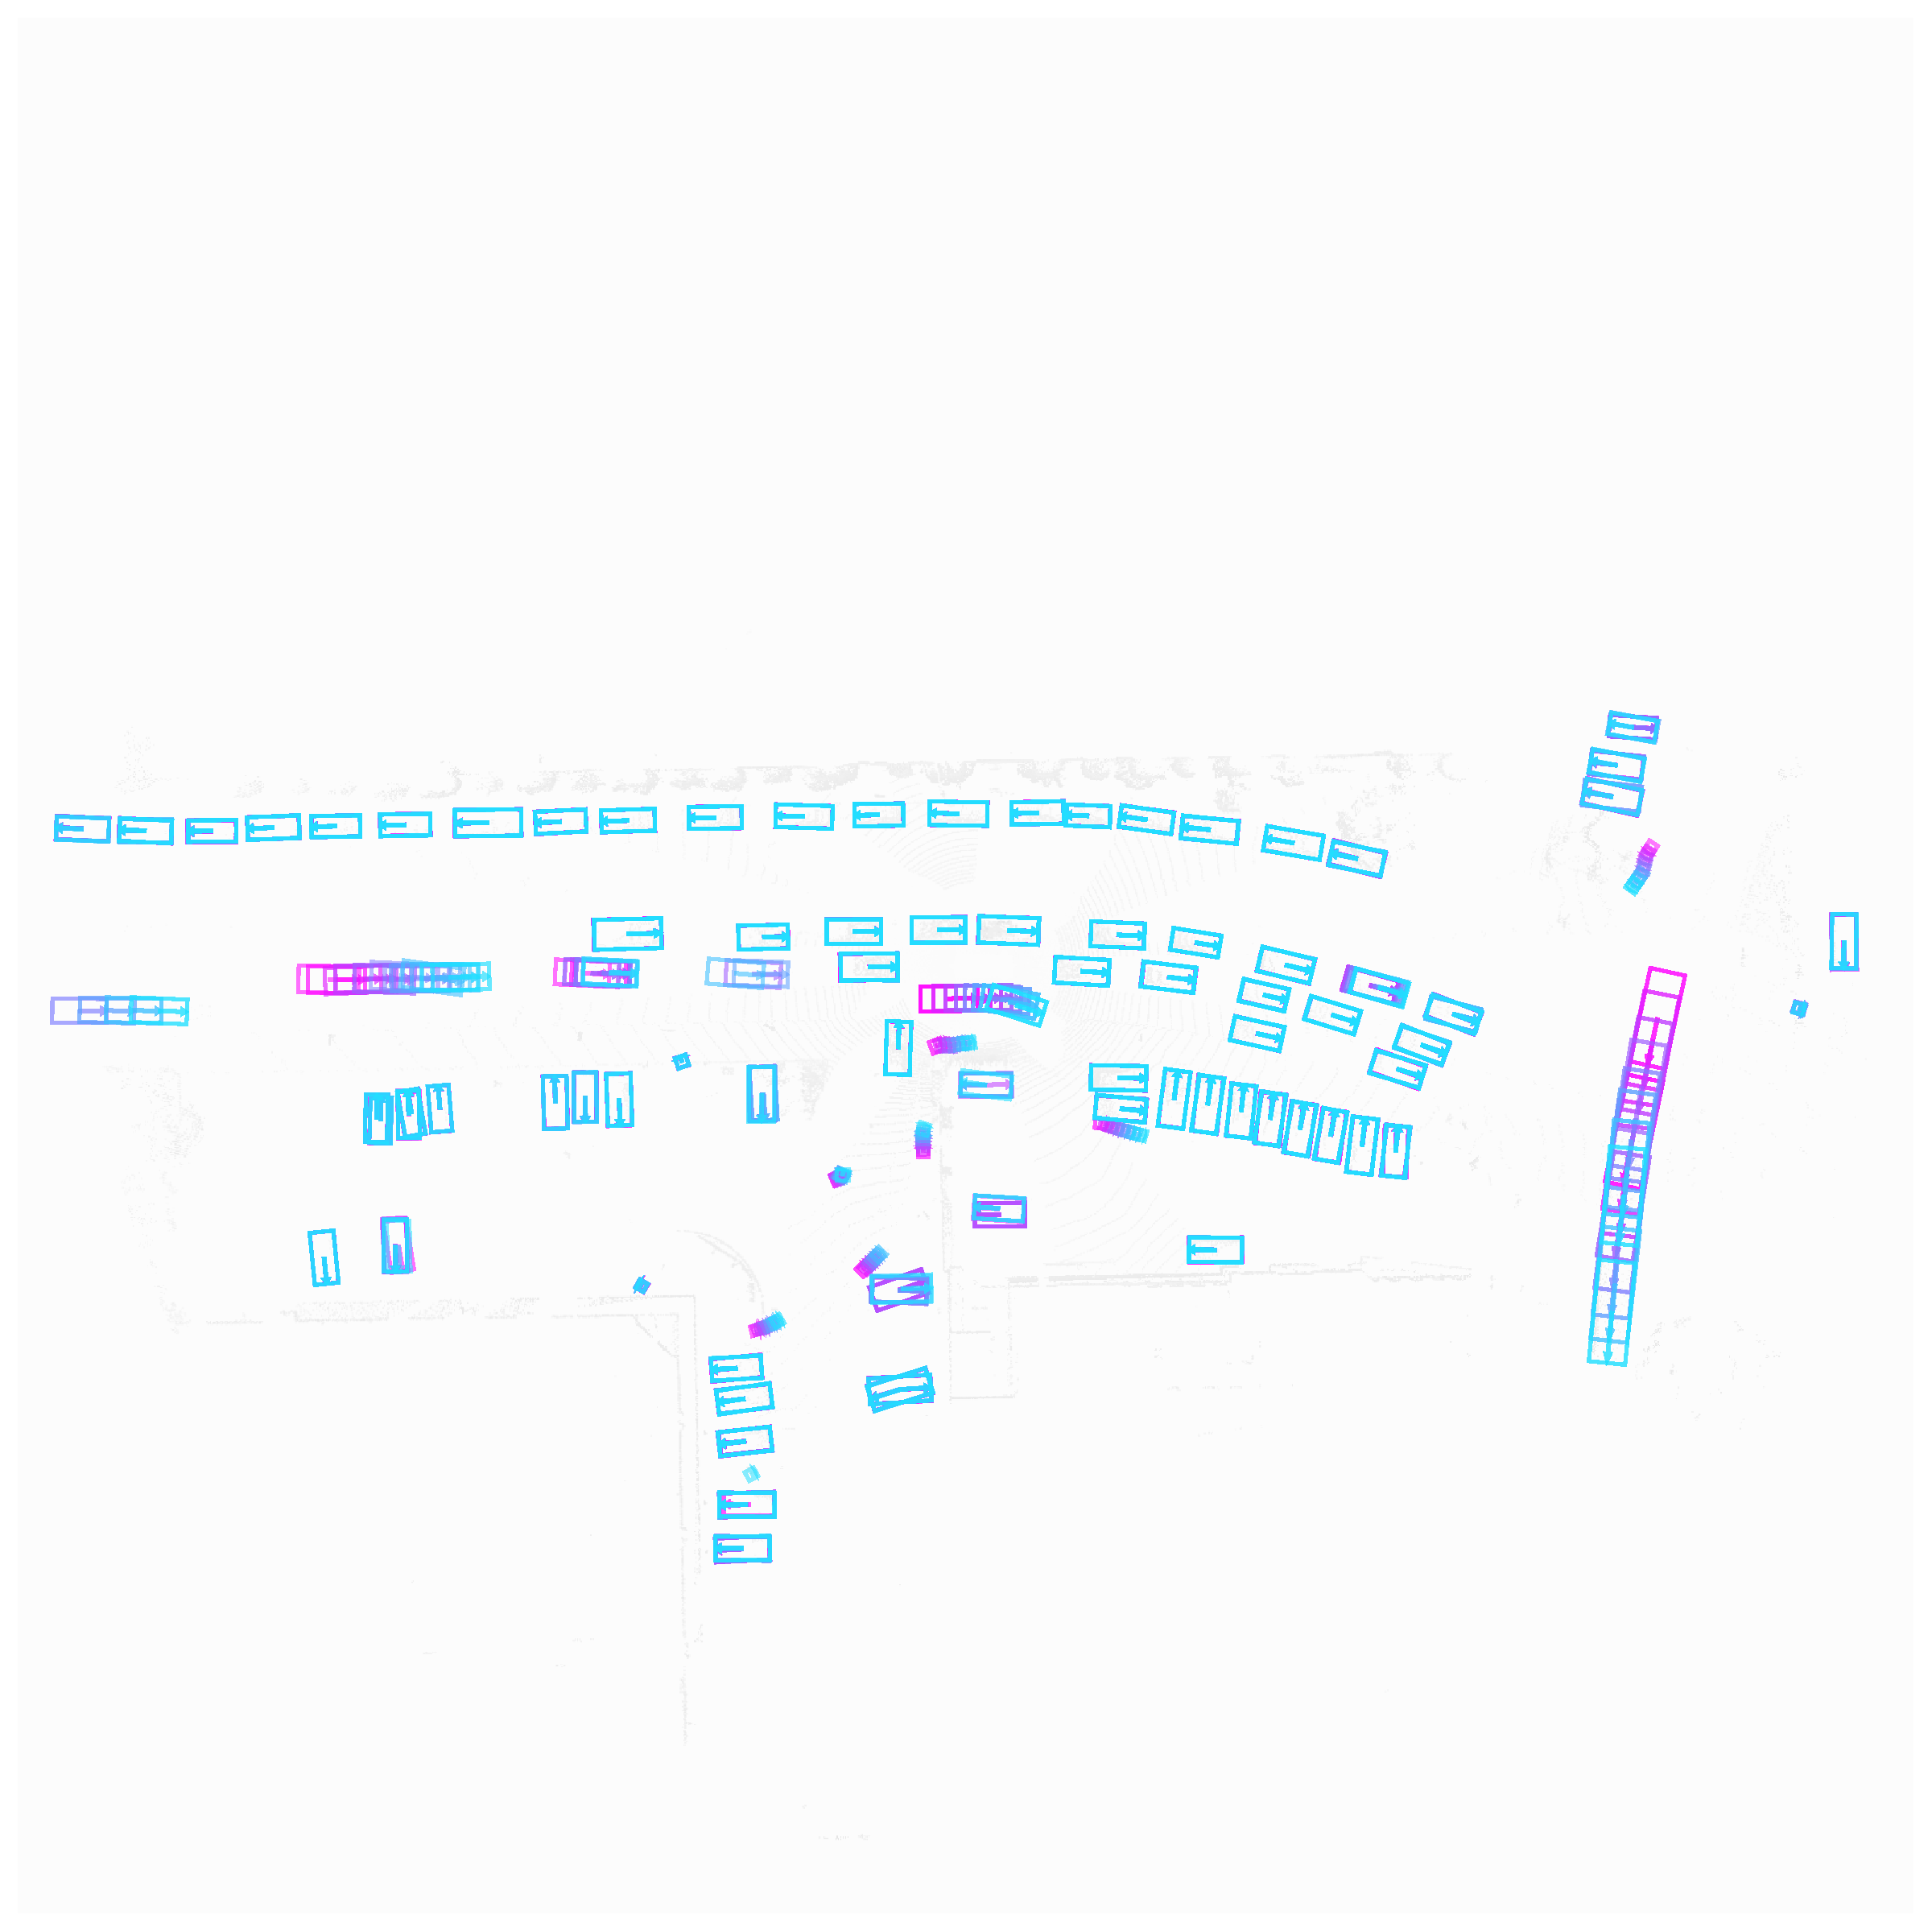
\includegraphics[width=\imw, viewport=396 216 1008 828, clip]{images/images_for_supp/31/original_det_anchors_wod_viz_31_198.pdf}};
        \node[draw=black,very thick,anchor=west , inner sep=0pt] (S5C) at (S5B.east)  {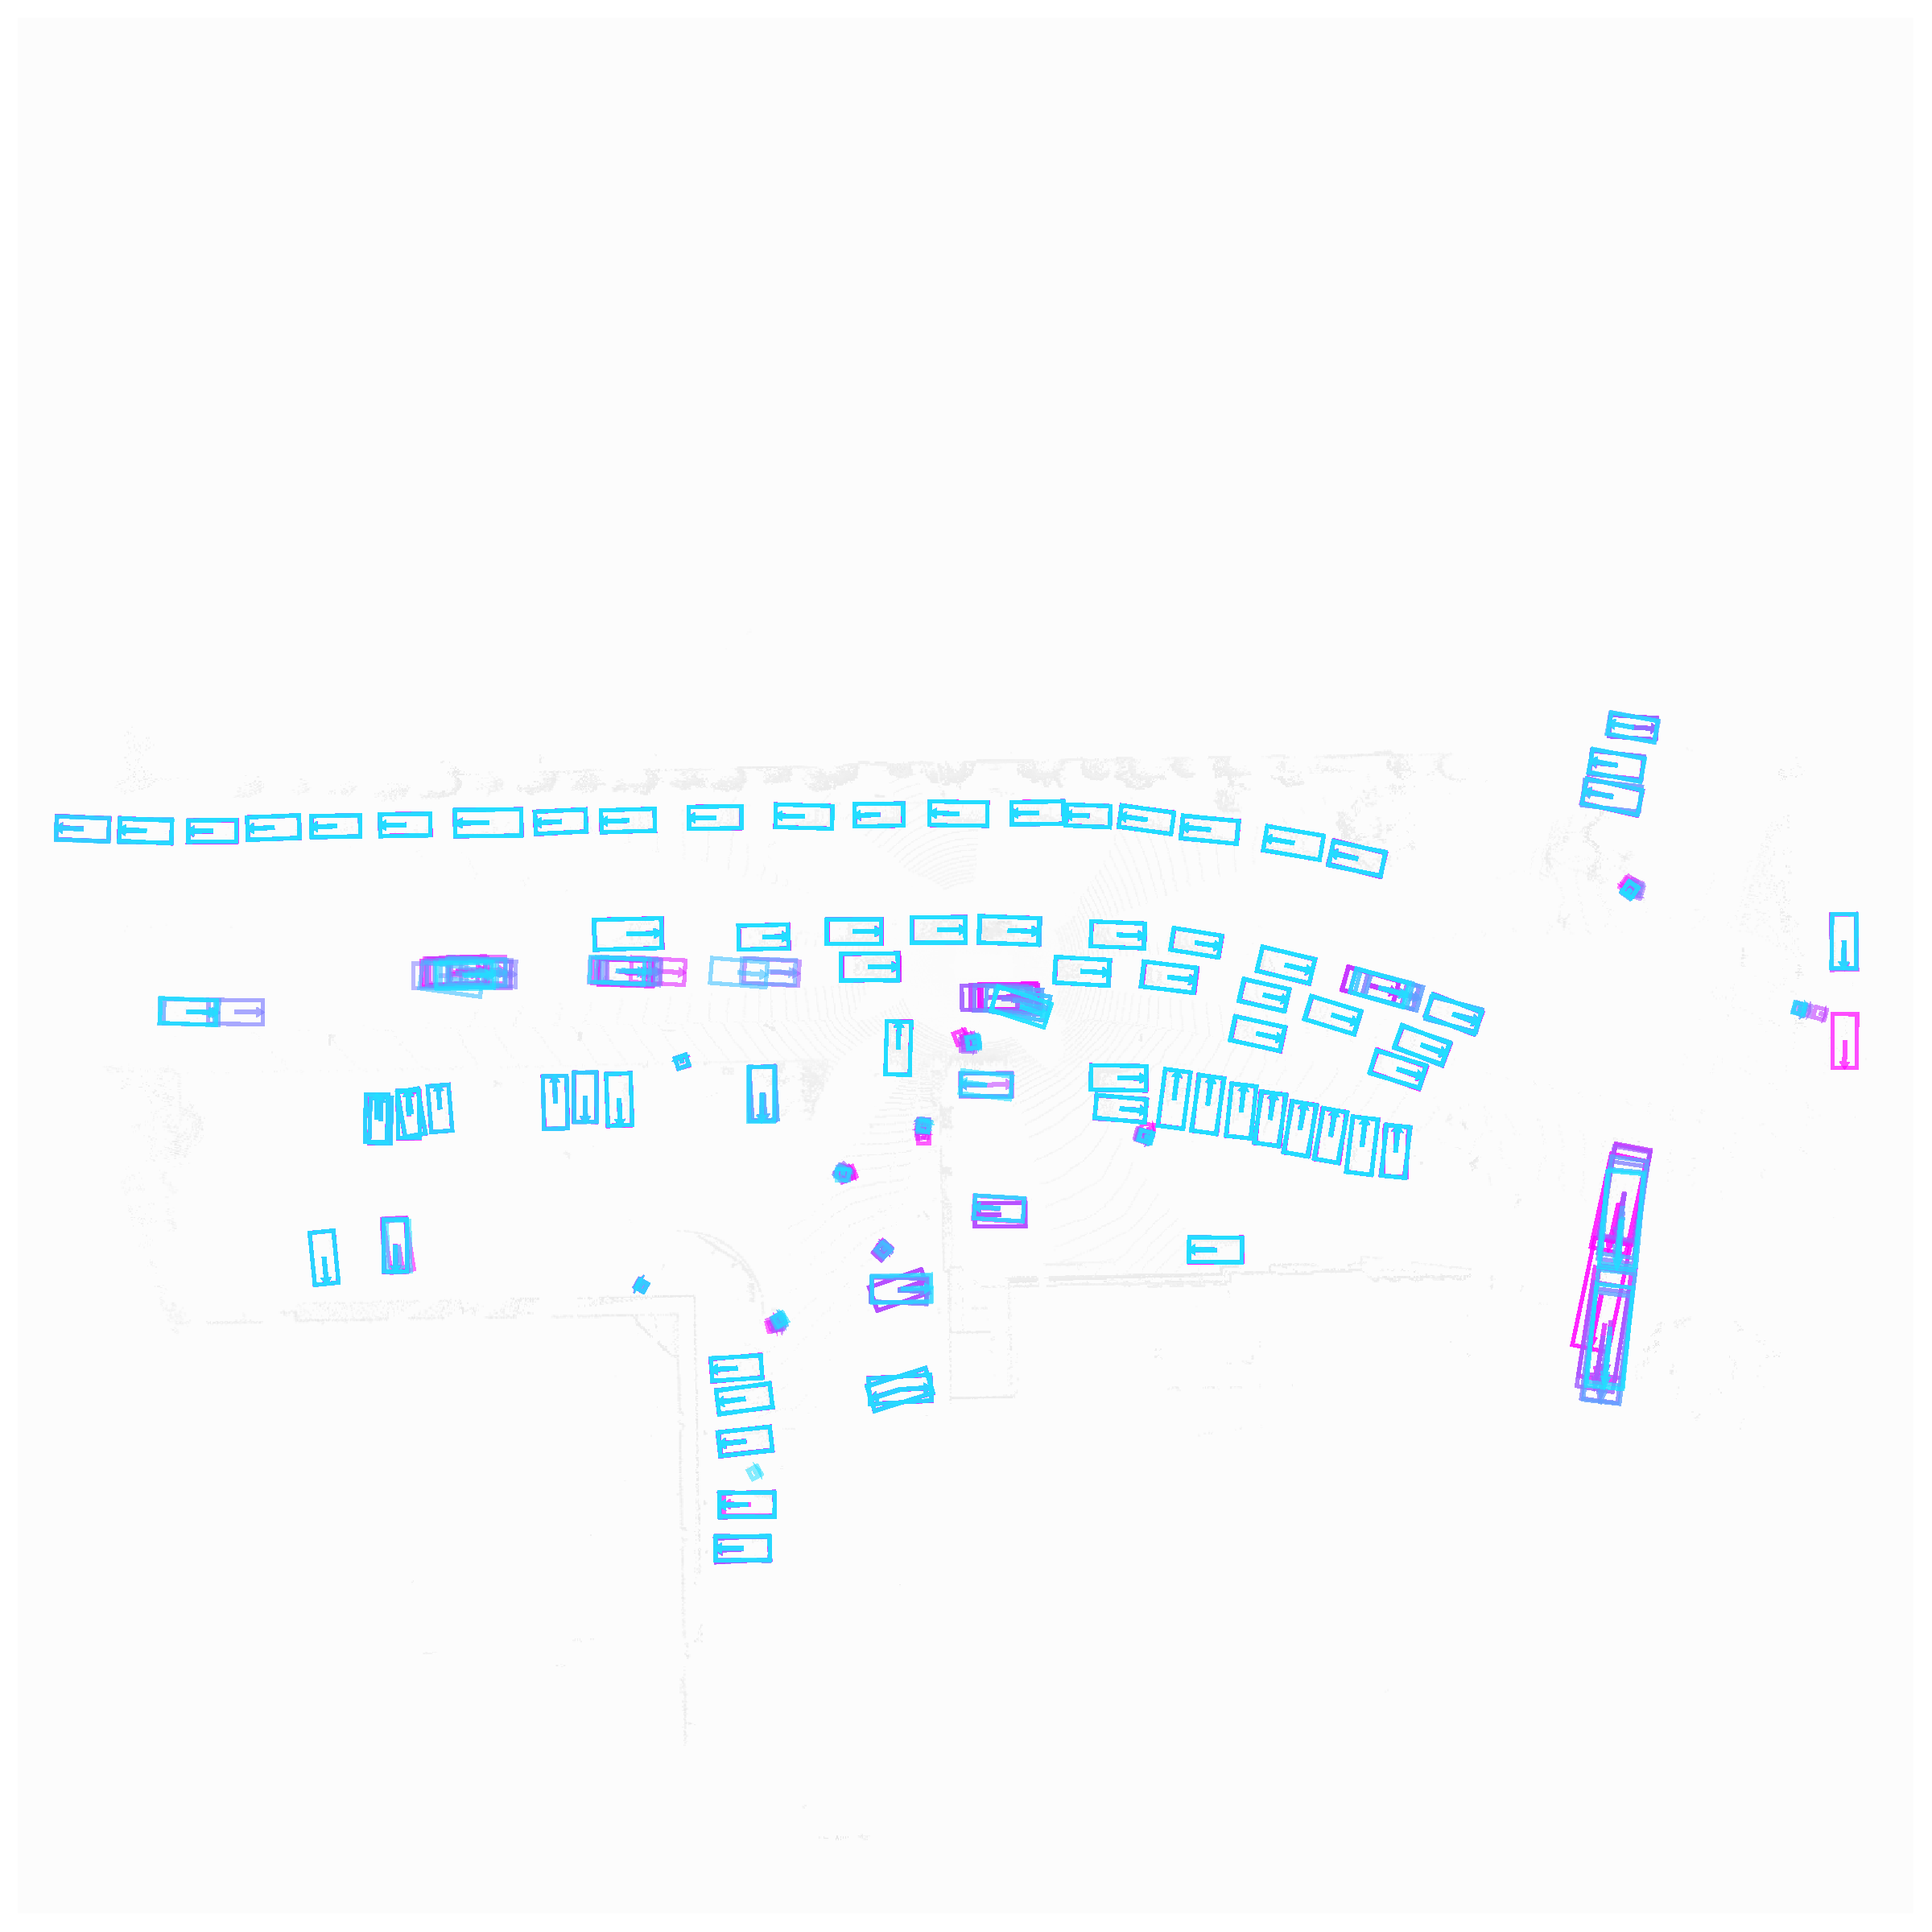
\includegraphics[width=\imw, viewport=396 216 1008 828, clip]{images/images_for_supp/31/interpolated_det_anchors_wod_viz_31_198.pdf}};
        \node[draw=black,very thick,anchor=west, inner sep=0pt] (S5A) at (S5C.east)      {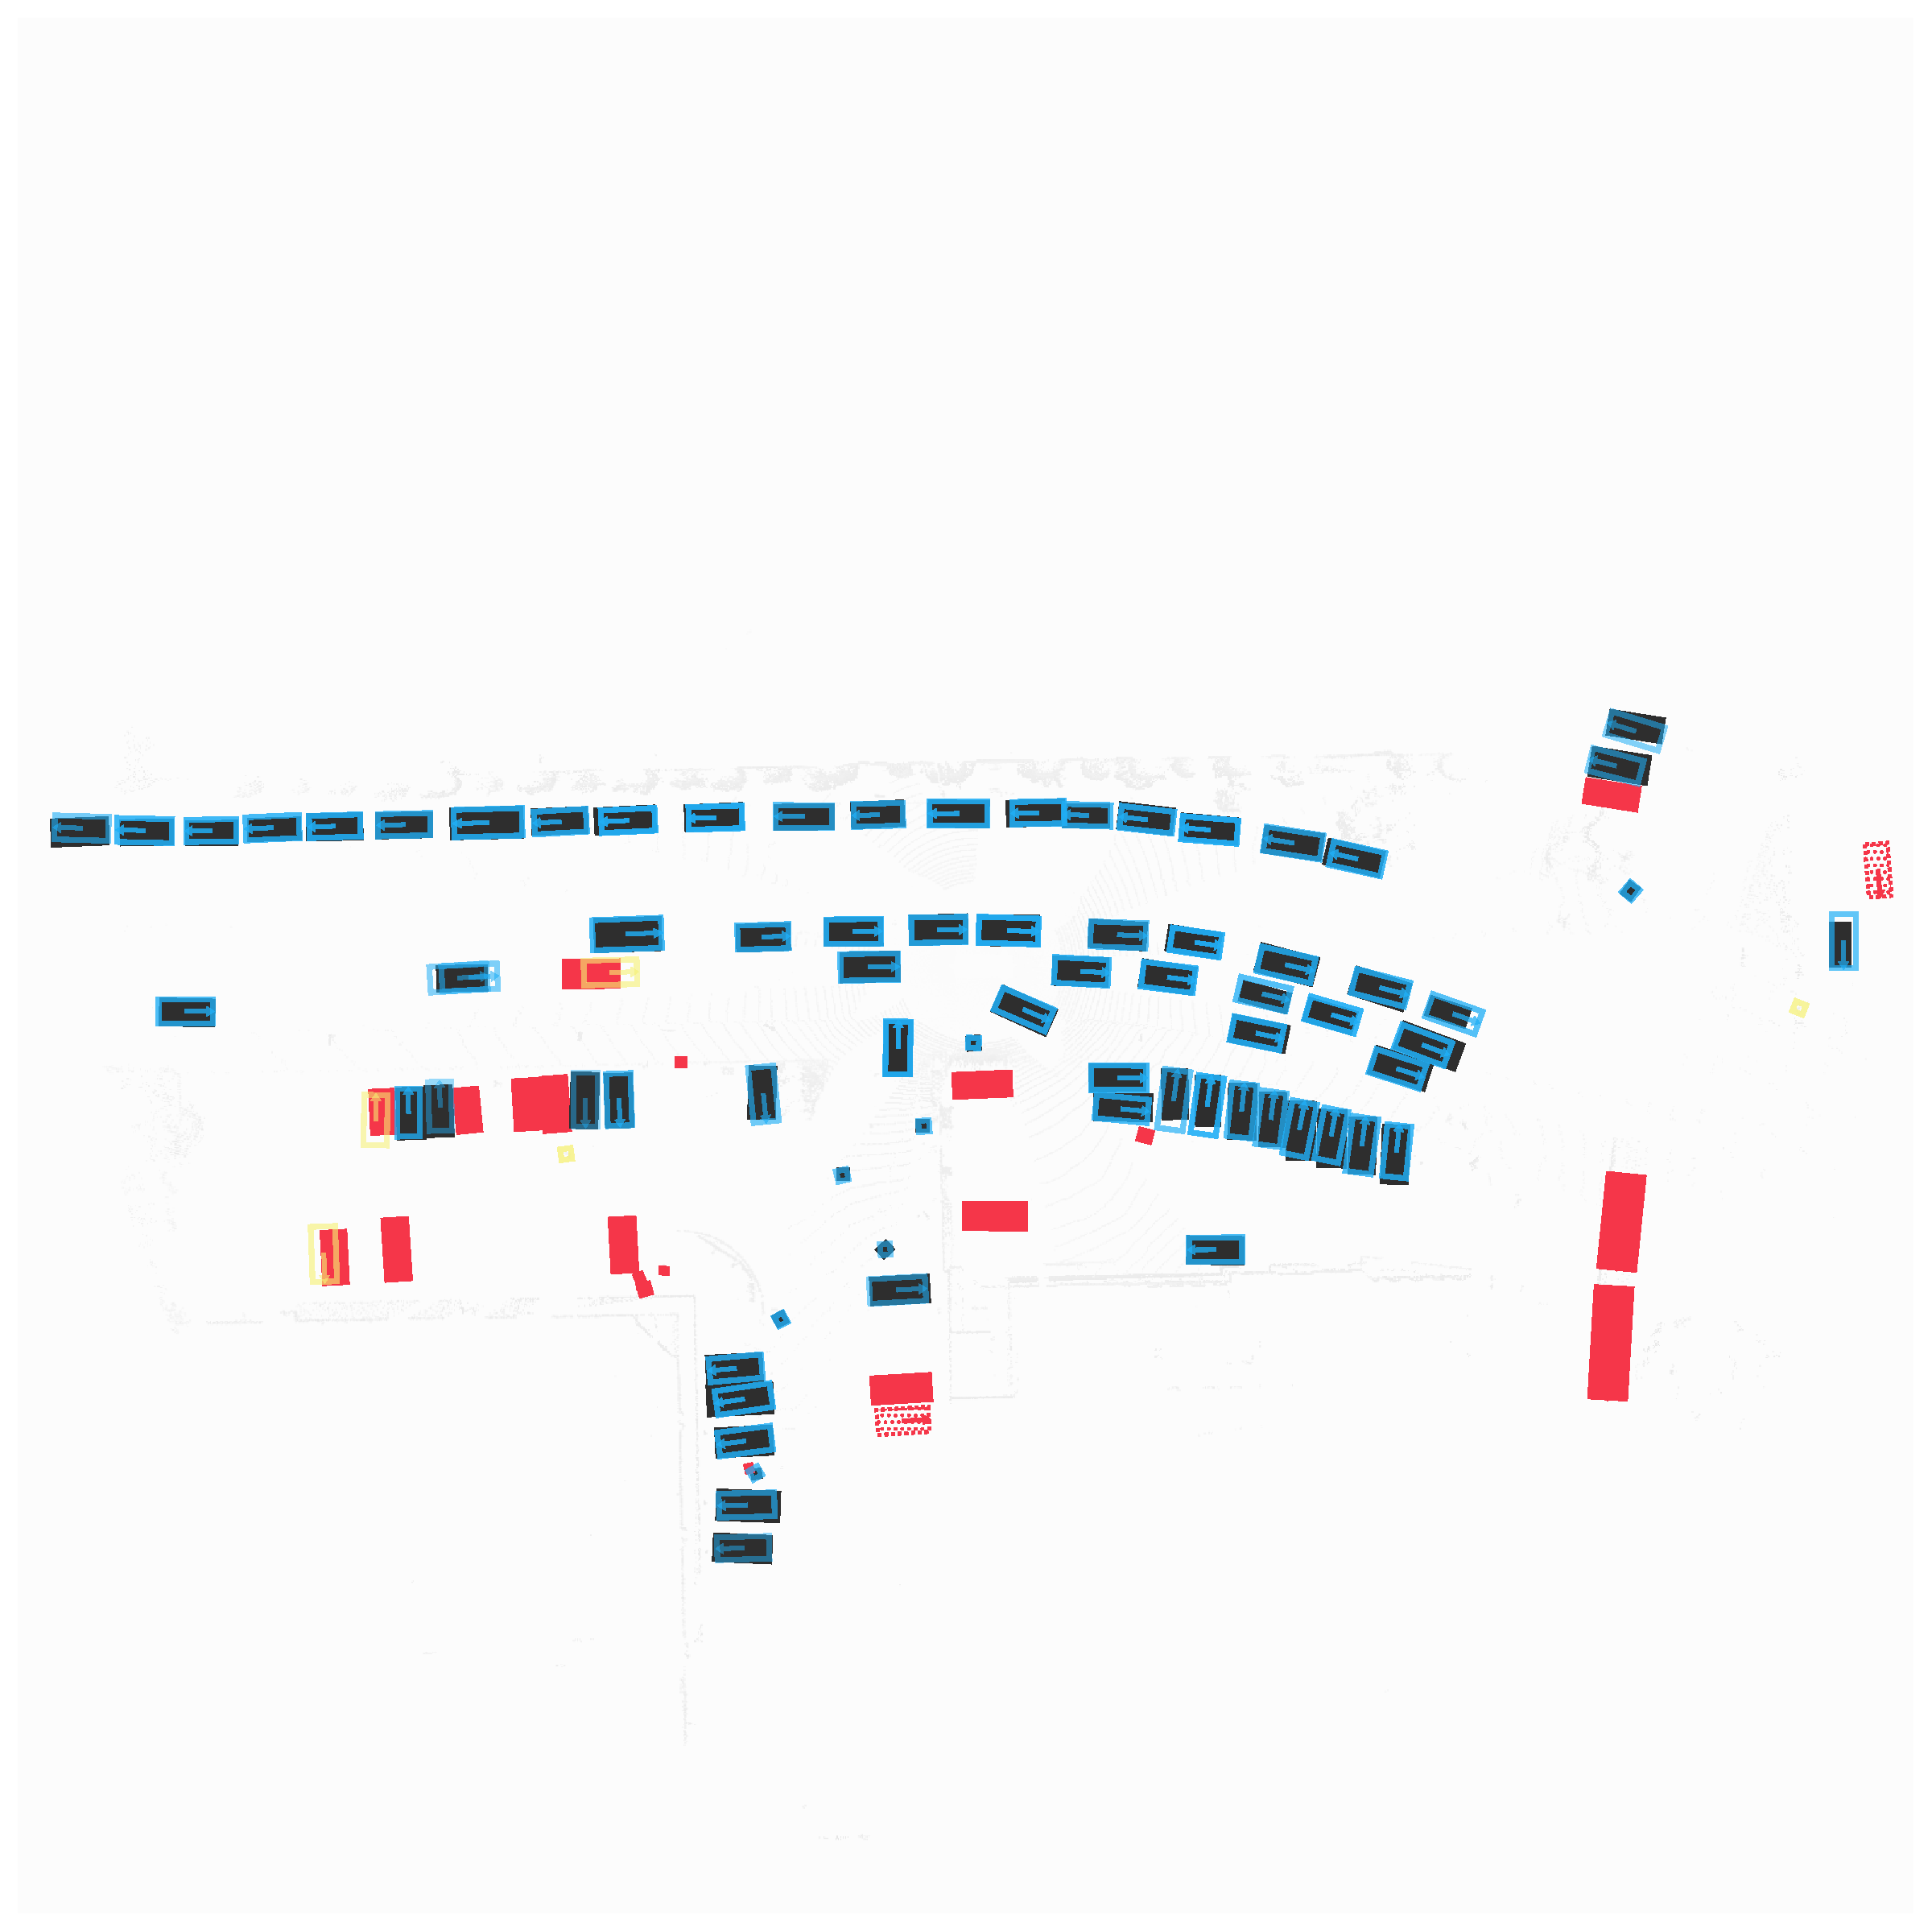
\includegraphics[width=\imw,  viewport=396 216 1008 828, clip]{images/images_for_supp/31/lidar_proposals_wod_viz_31_198.pdf}};
        \node[draw=black,very thick,anchor=west , inner sep=0pt] (S5D) at (S5A.east)  {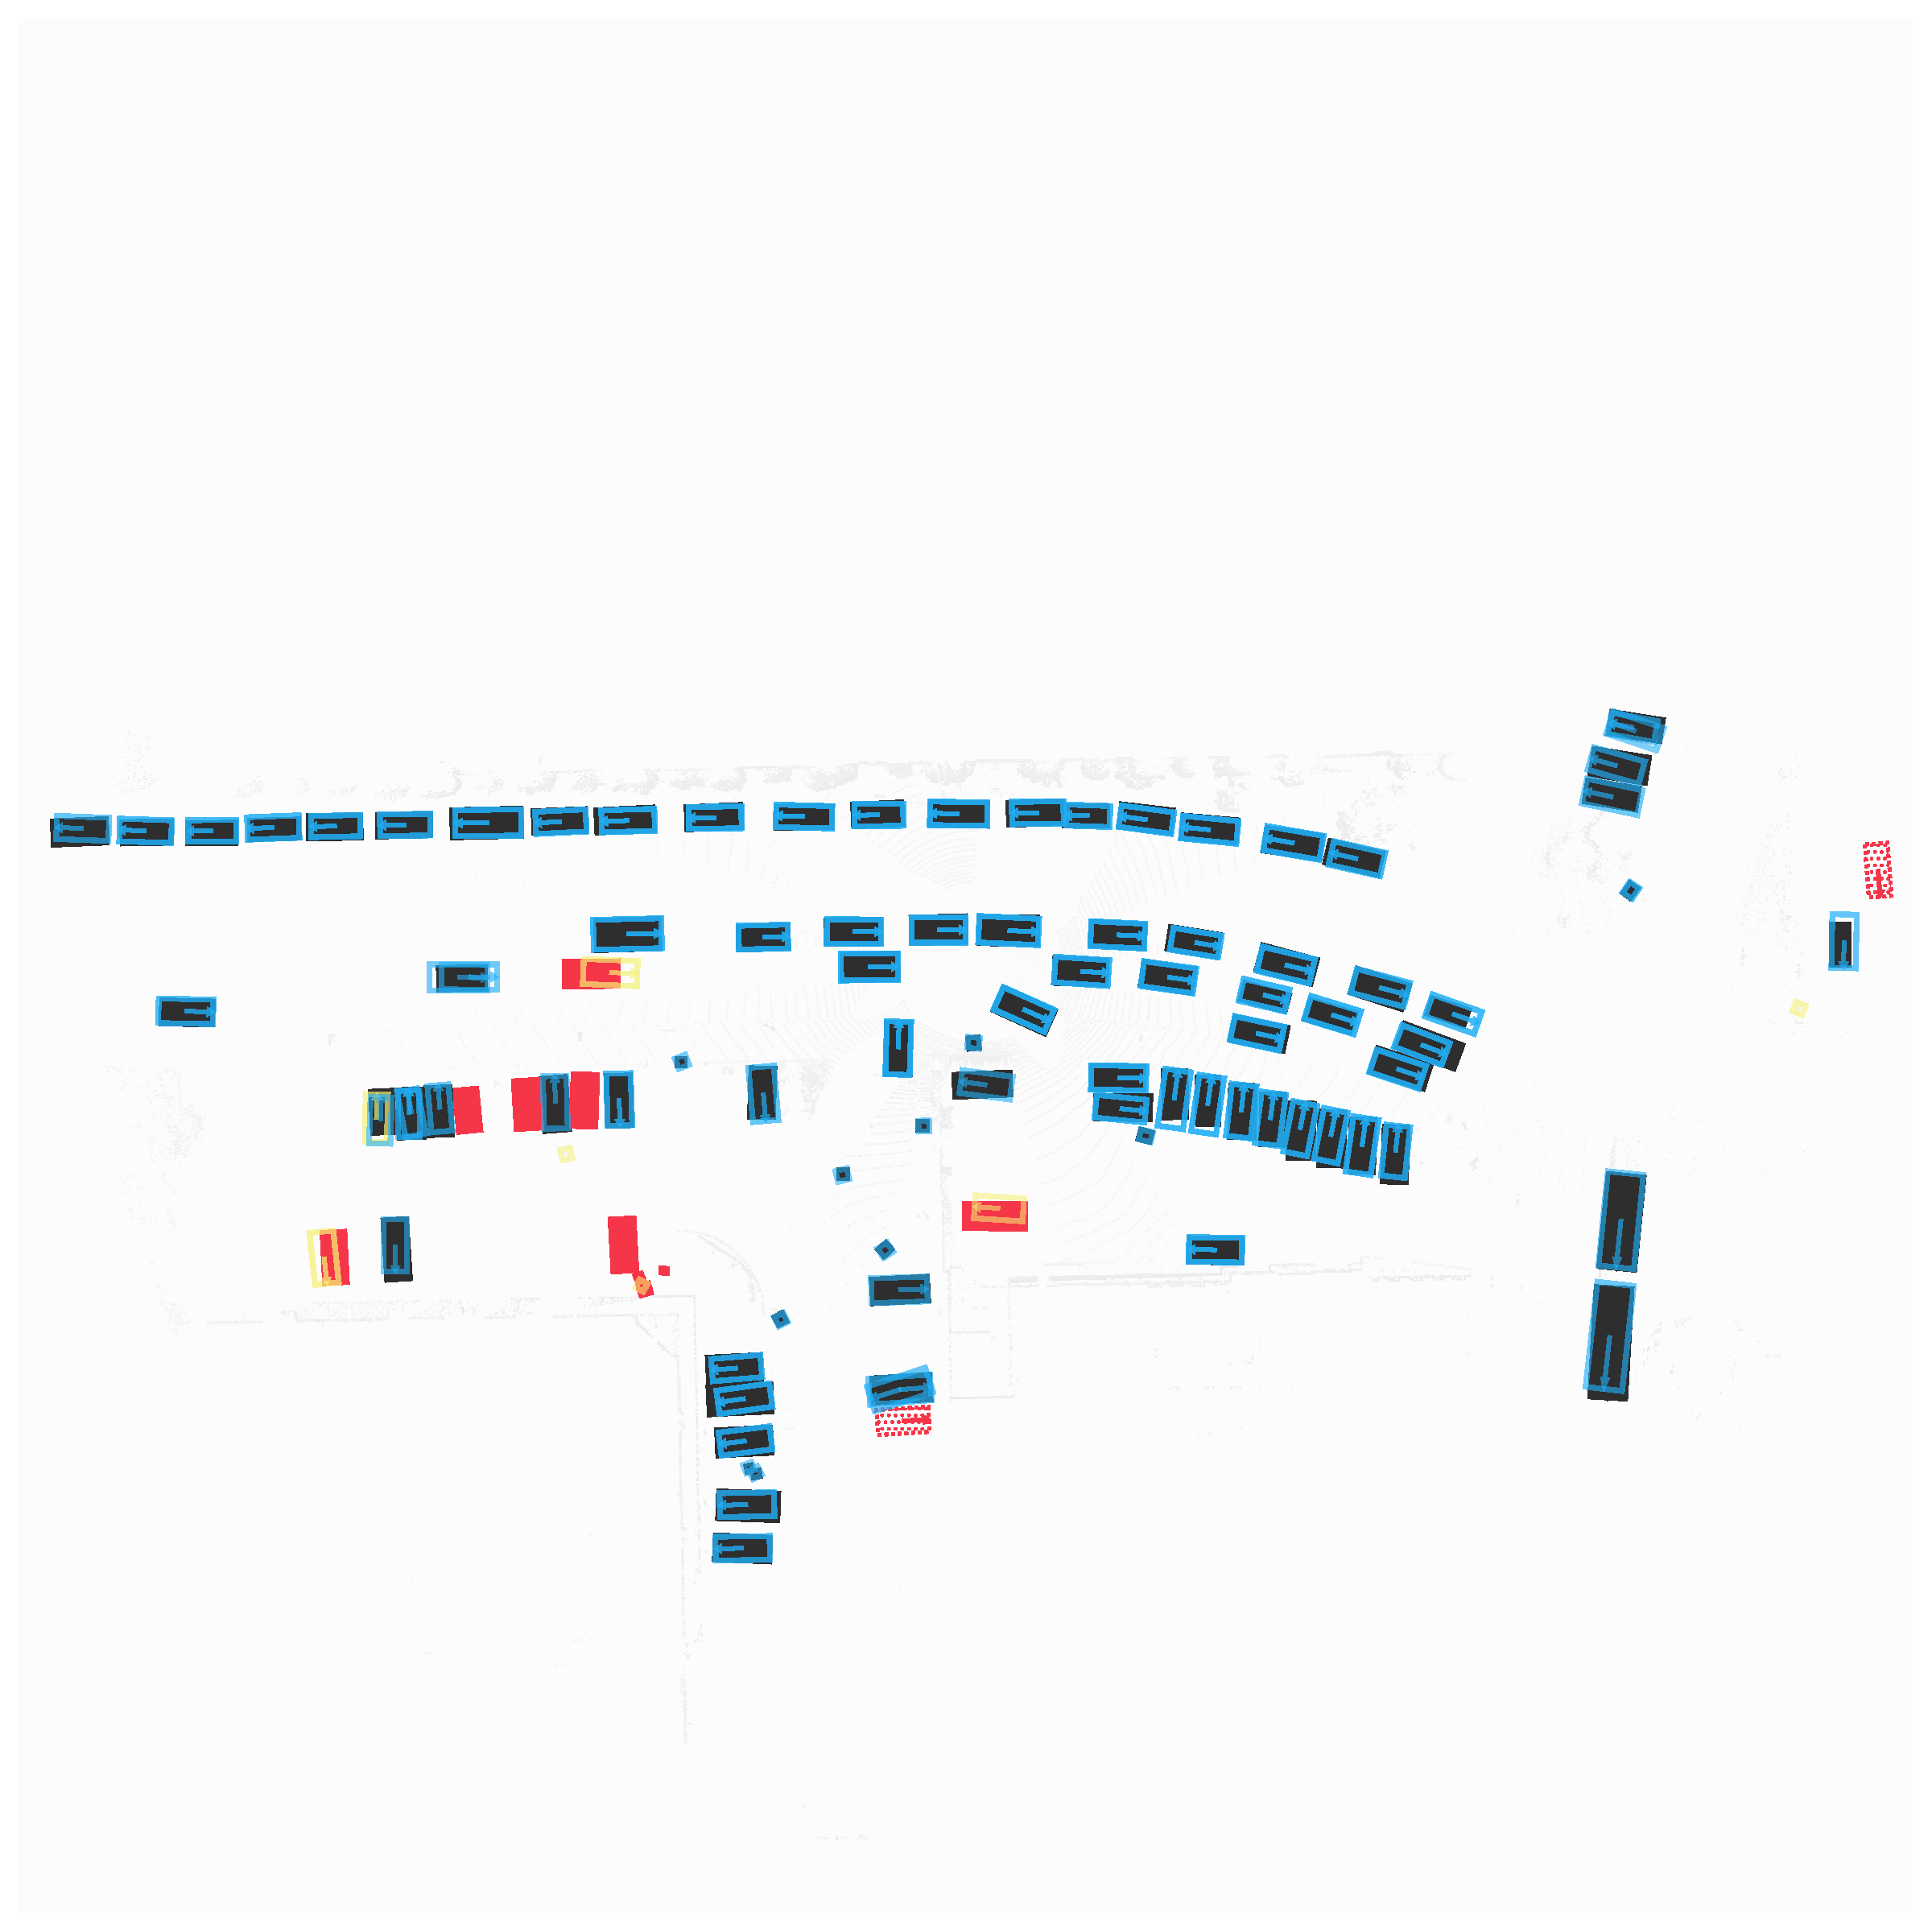
\includegraphics[width=\imw, viewport=396 216 1008 828, clip]{images/images_for_supp/31/detections_wod_viz_31_198.pdf}};
    
        \node at (S5A.north) [anchor=south] {\footnotesize Detection Proposal Boxes $\mathbf{B}^\mathrm{det}$};
        \node at (S5B.north) [anchor=south] {\footnotesize Memory Bank};
        \node at (S5C.north) [anchor=south] {\footnotesize Memory Proposal Boxes $\mathbf{B}^\mathrm{mem}$};
        \node at (S5D.north) [anchor=south] {\footnotesize \ourmodel{} Output Boxes $\mathbf{B}^\mathrm{ref}$};
    
        \node[draw=black,very thick,anchor=north , inner sep=0pt]  (S6B) at ([yshift=-\rowsep]S5B.south)                   {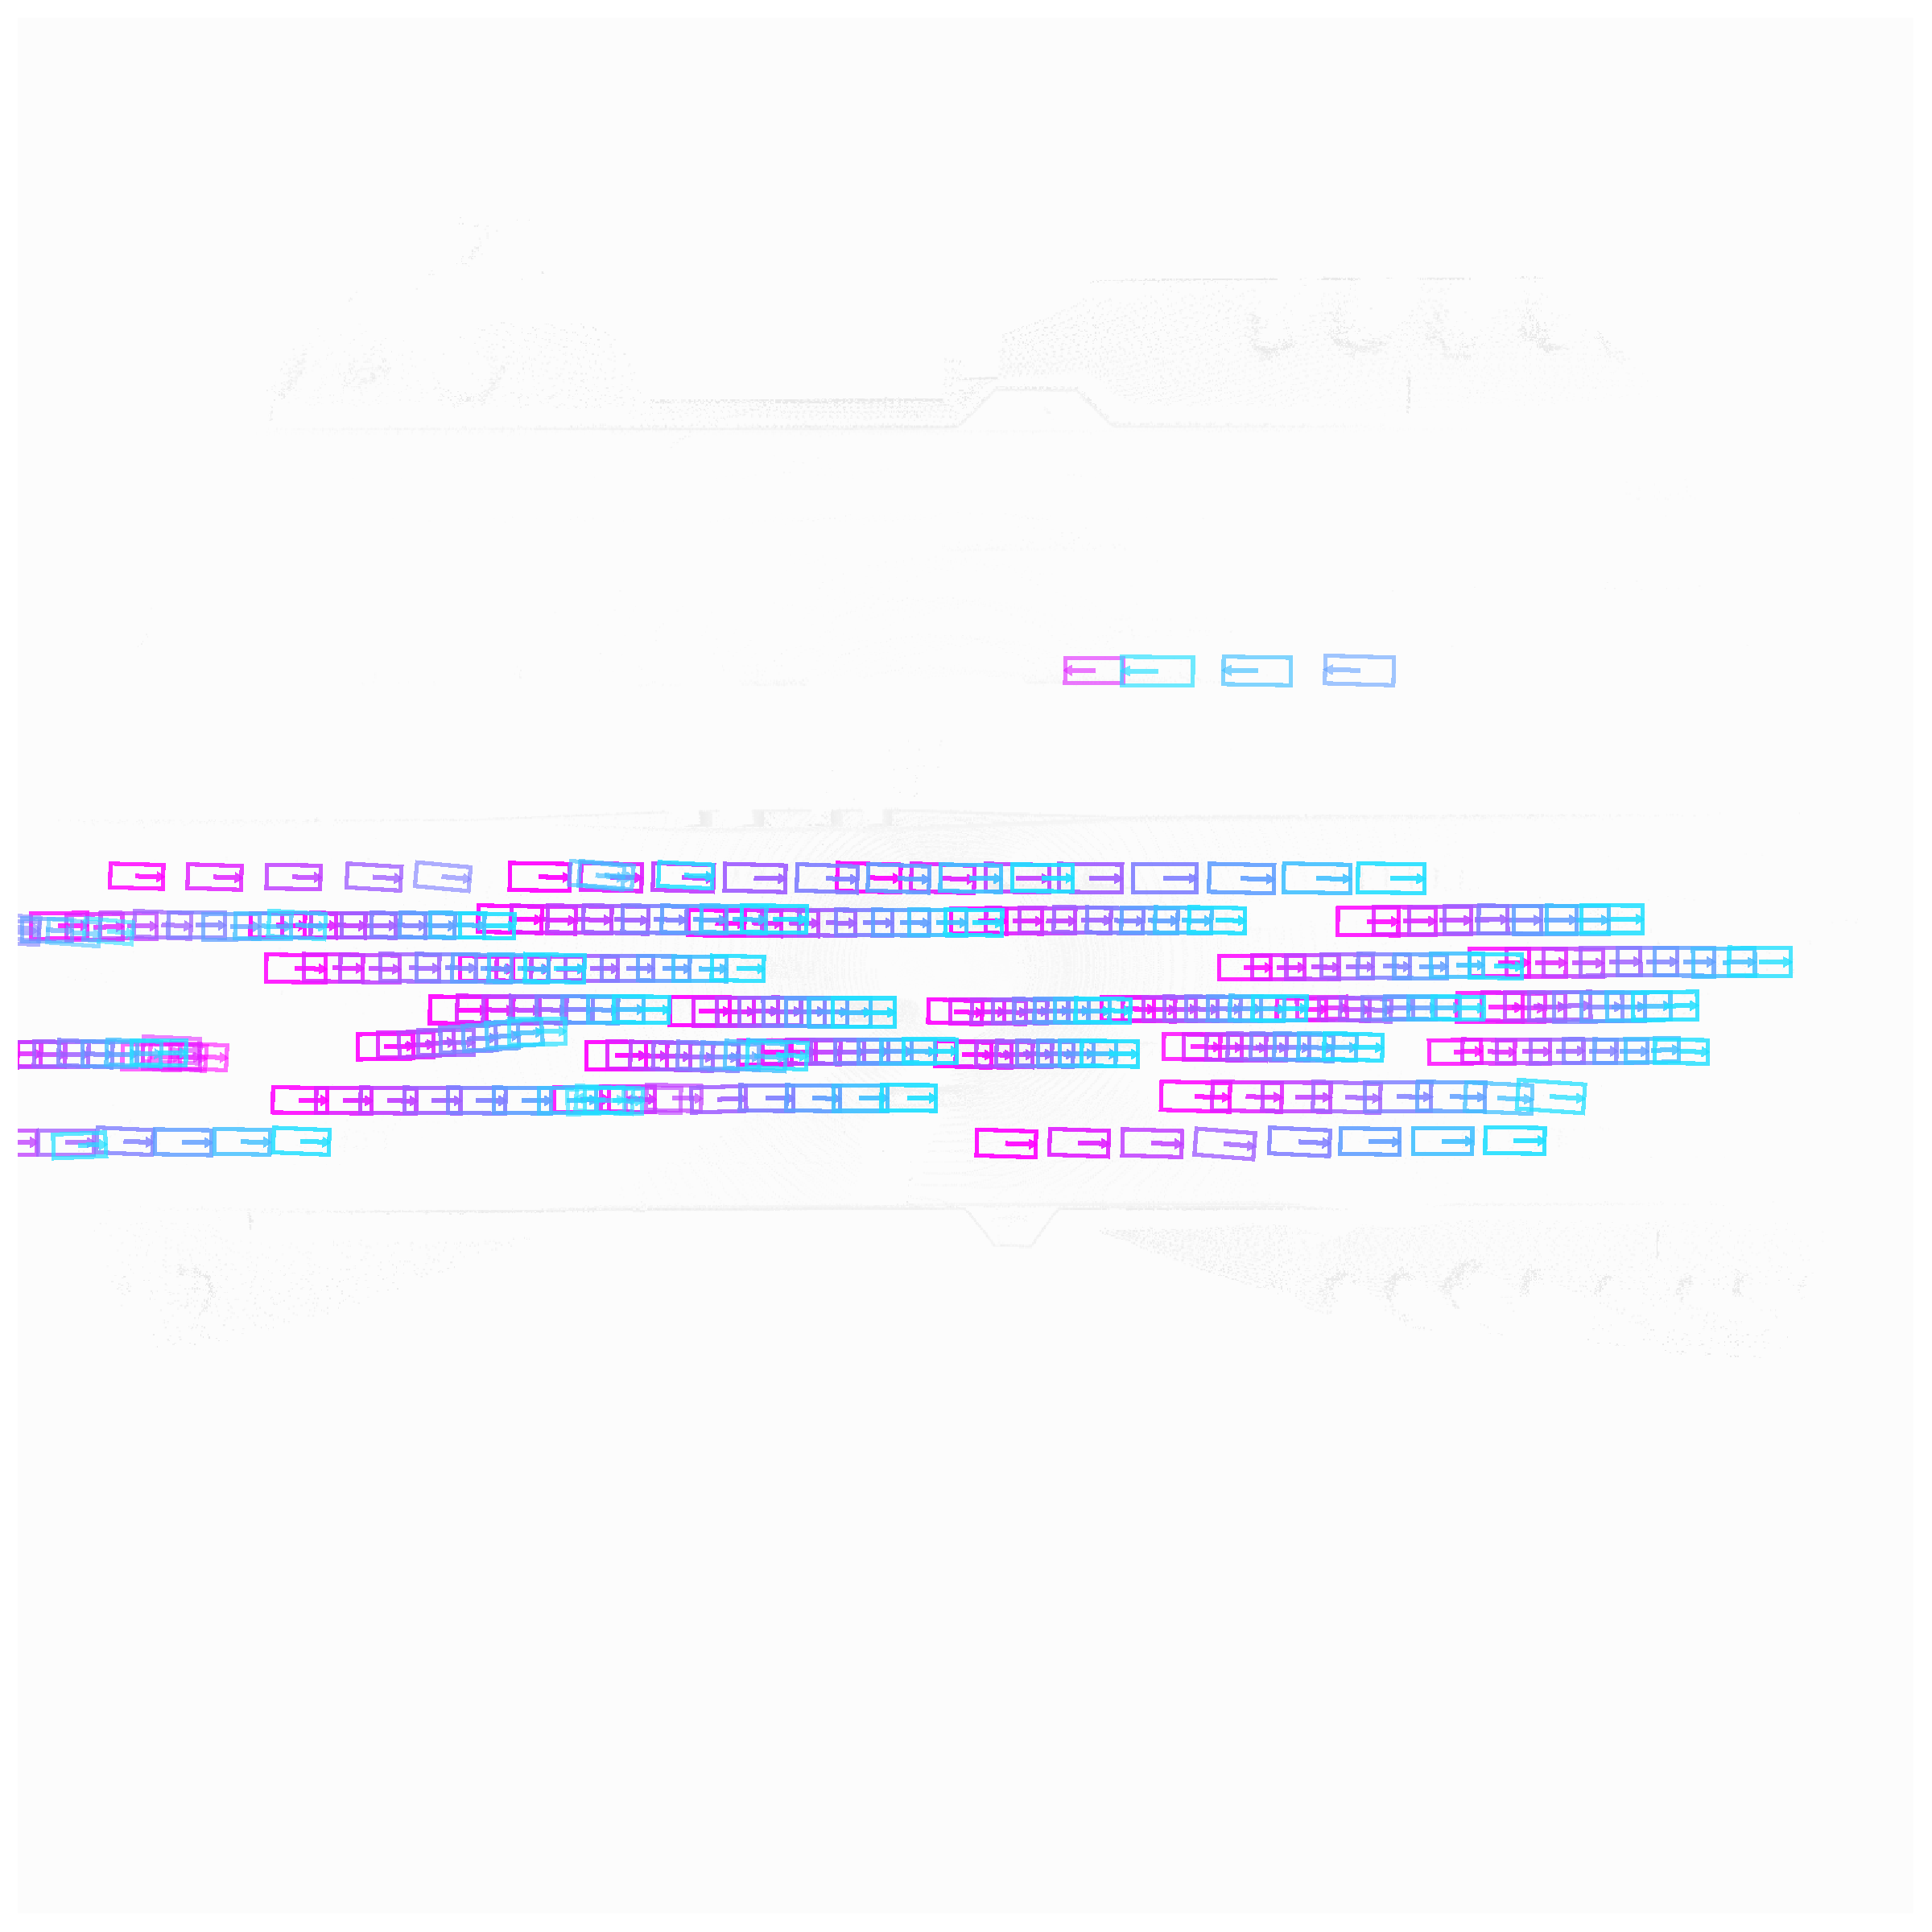
\includegraphics[width=\imw, viewport=10 270 480 740, clip]{images/images_for_supp/82/original_det_anchors_wod_viz_82_120.pdf}};
        \node[draw=black,very thick,anchor=west , inner sep=0pt]  (S6C) at (S6B.east)                   {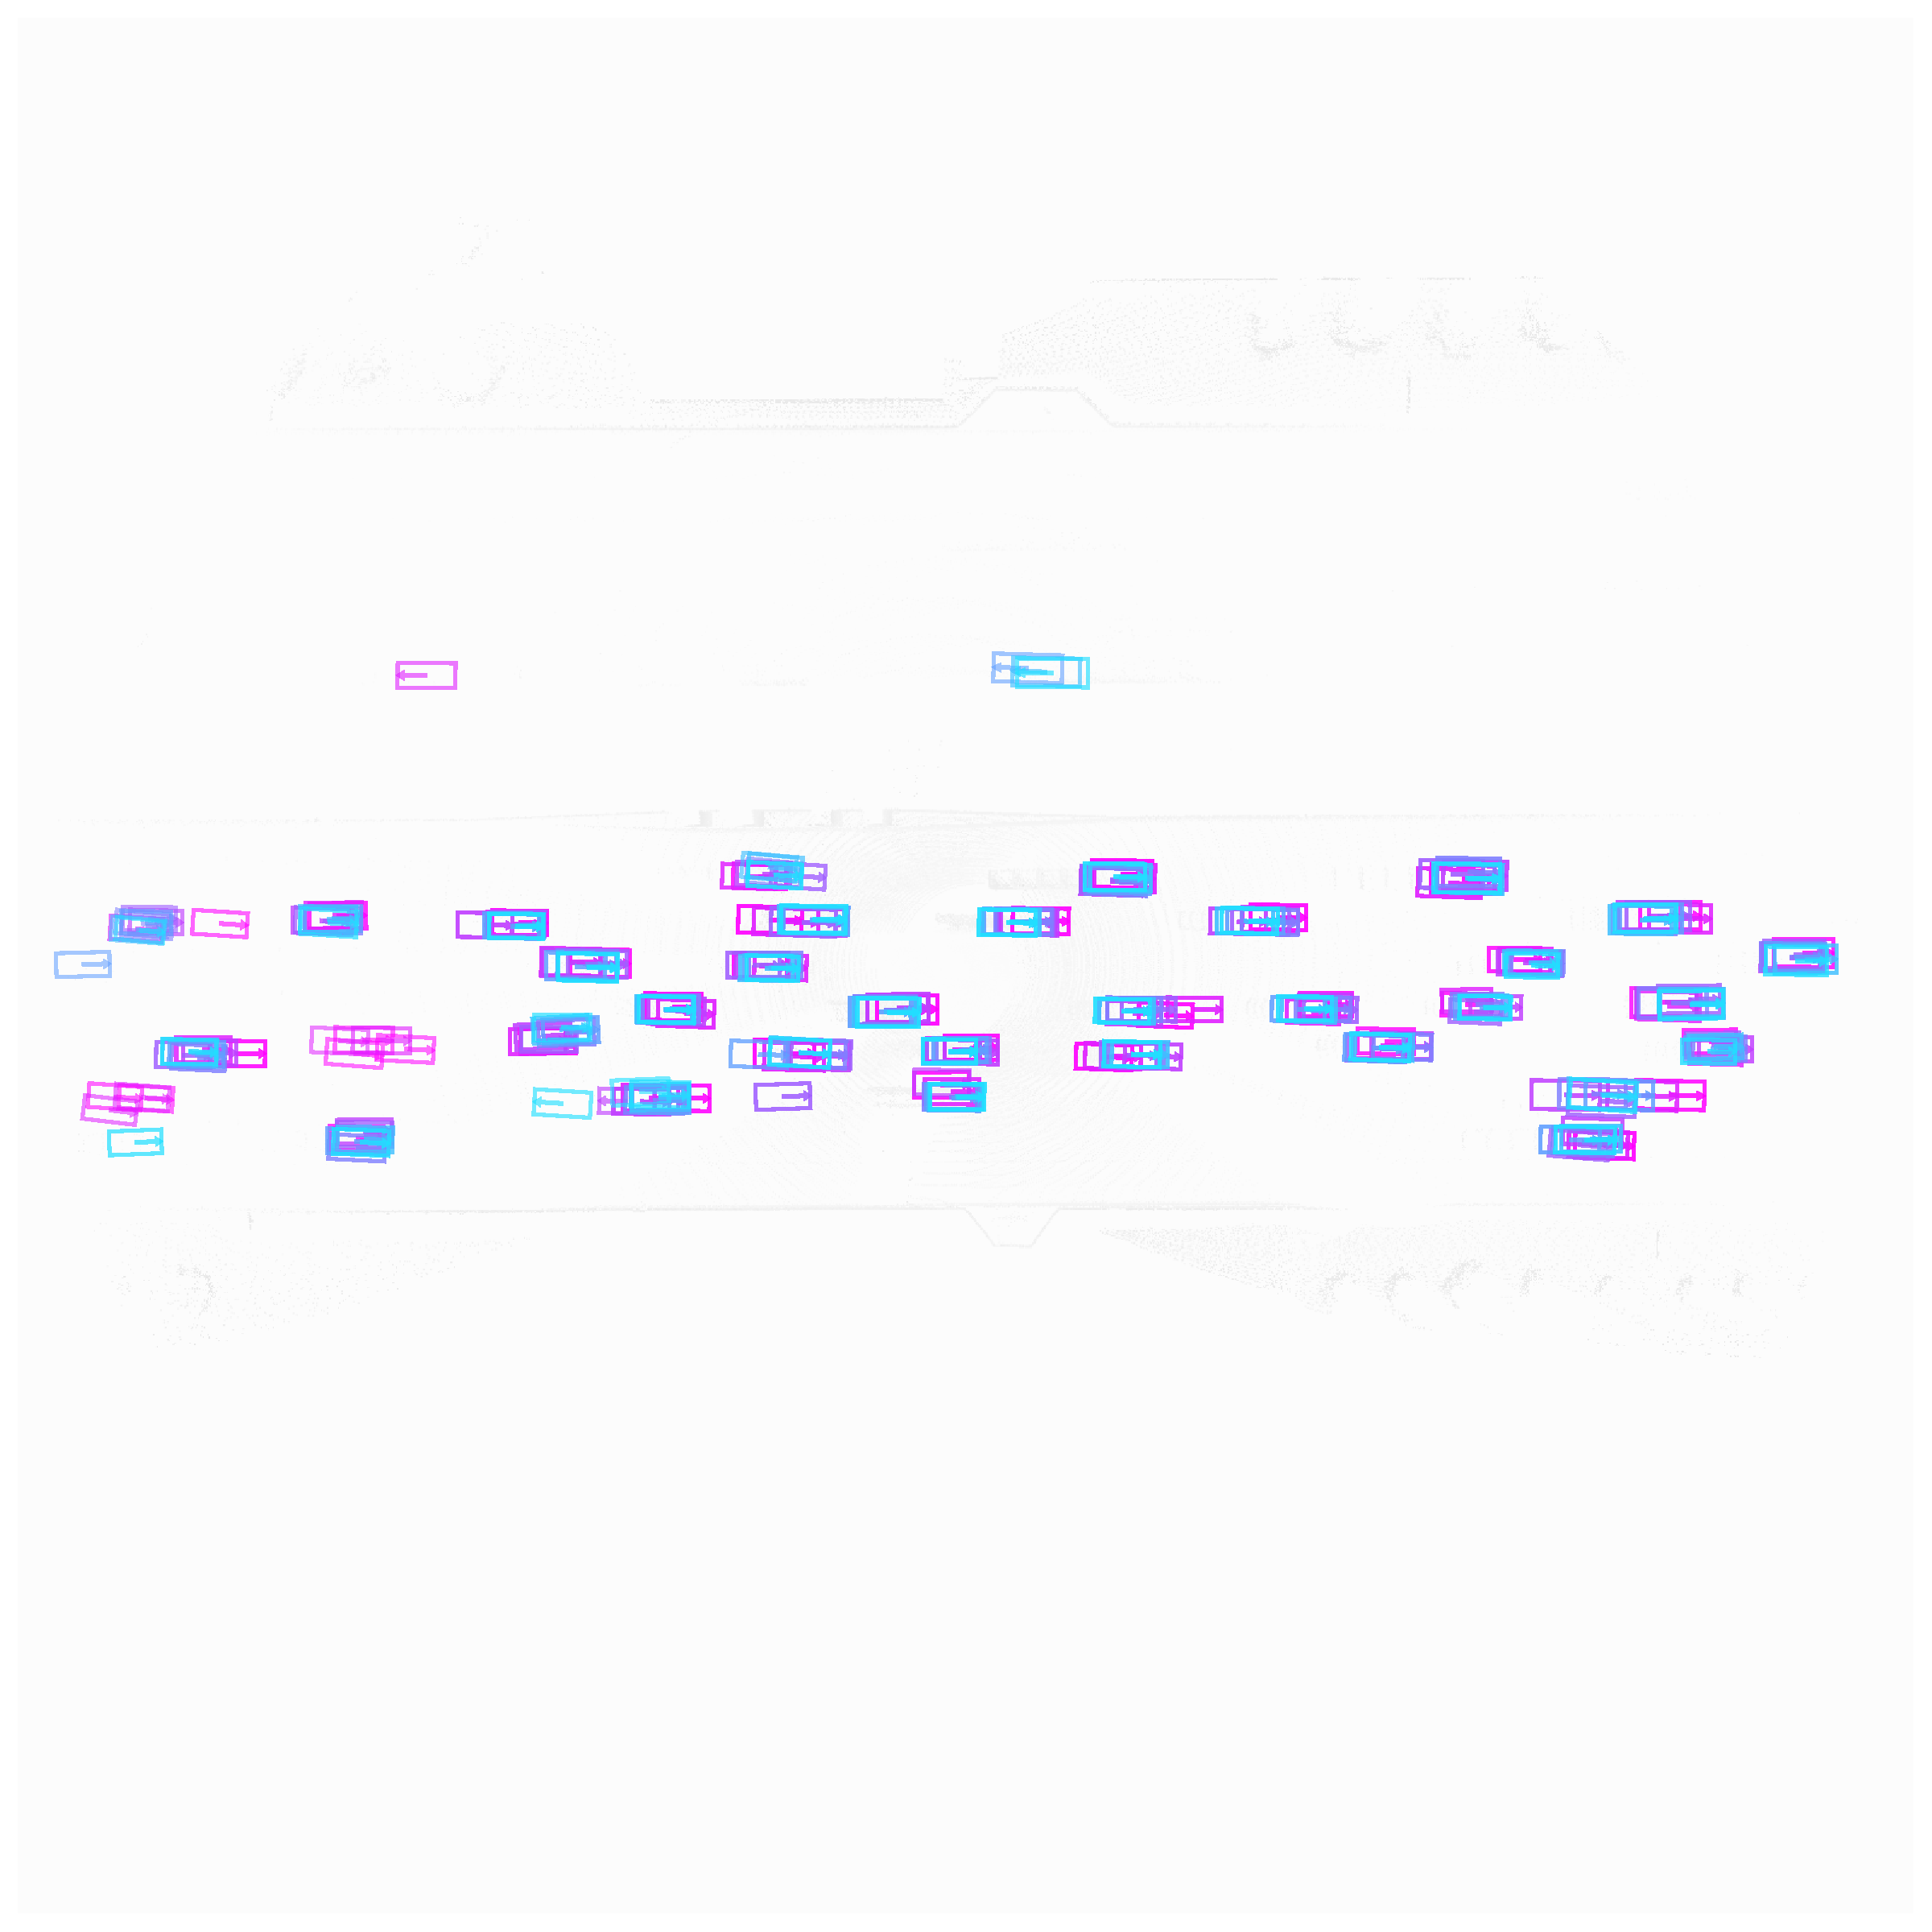
\includegraphics[width=\imw, viewport=10 270 480 740, clip]{images/images_for_supp/82/interpolated_det_anchors_wod_viz_82_120.pdf}};
        \node[draw=black,very thick,anchor=west, inner sep=0pt] (S6A) at (S6C.east) {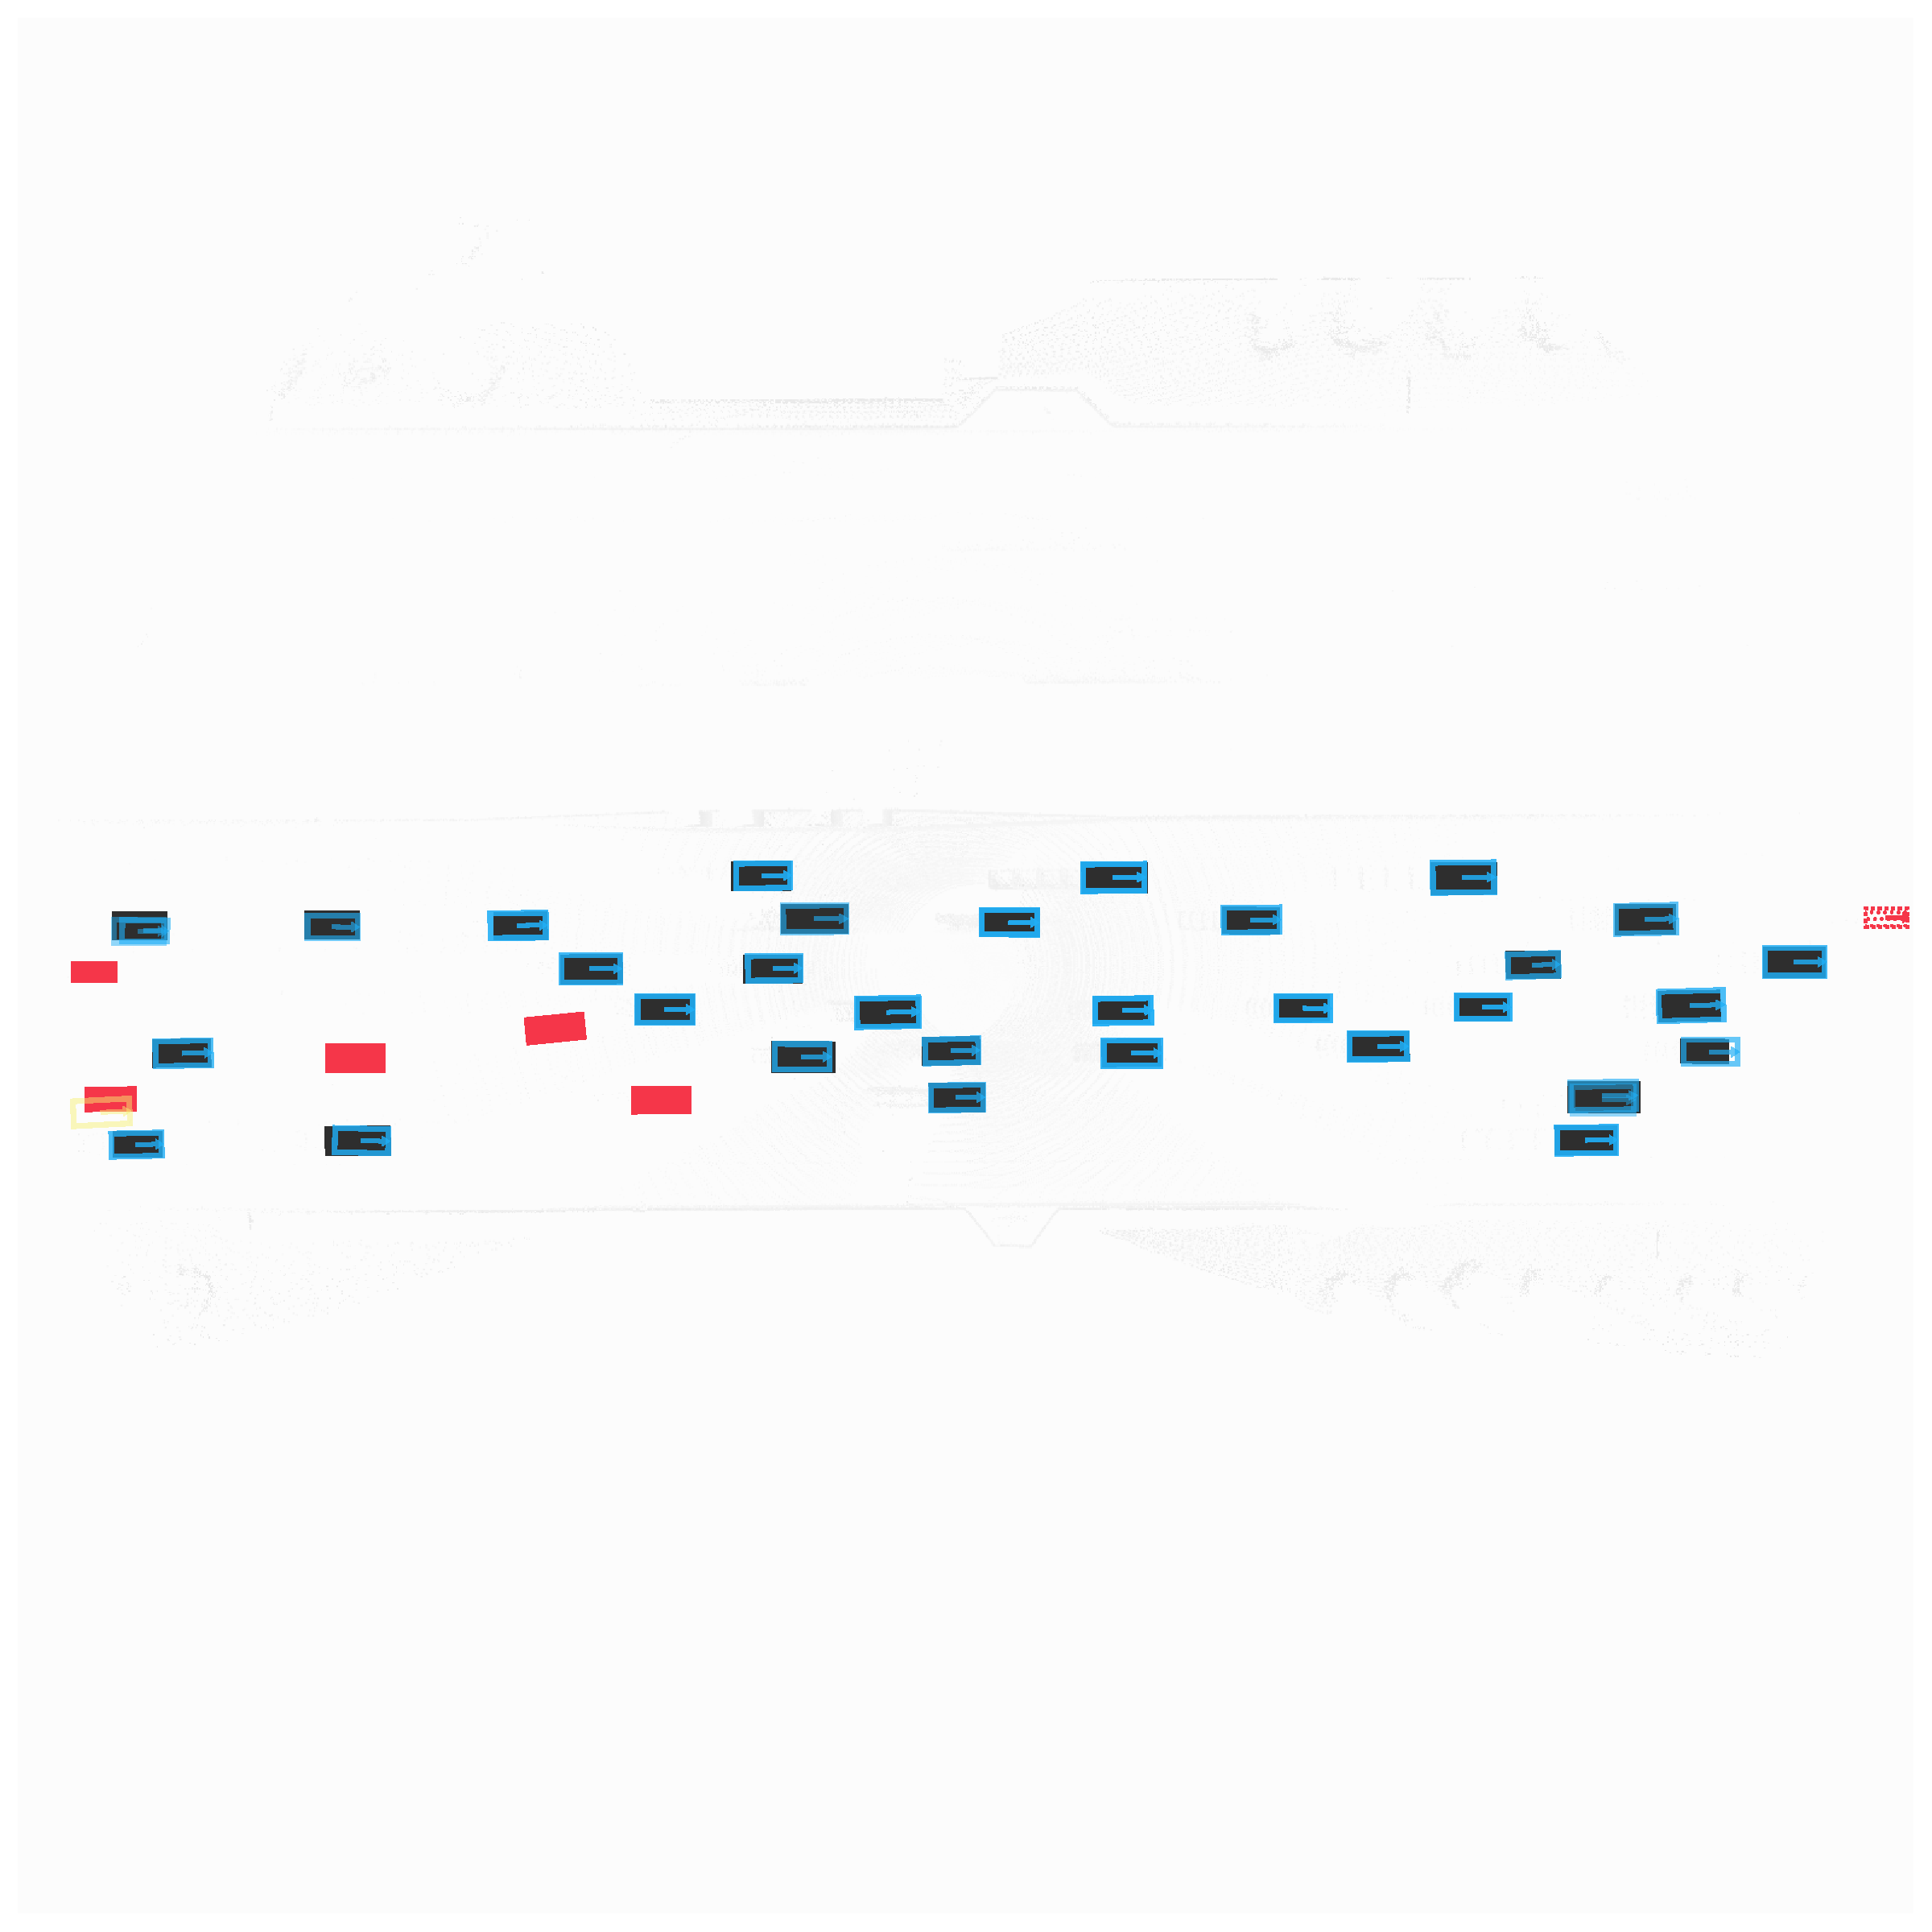
\includegraphics[width=\imw, viewport= 10 270 480 740, clip] {images/images_for_supp/82/lidar_proposals_wod_viz_82_120.pdf}};
        \node[draw=black,very thick,anchor=west , inner sep=0pt]  (S6D) at (S6A.east)                   {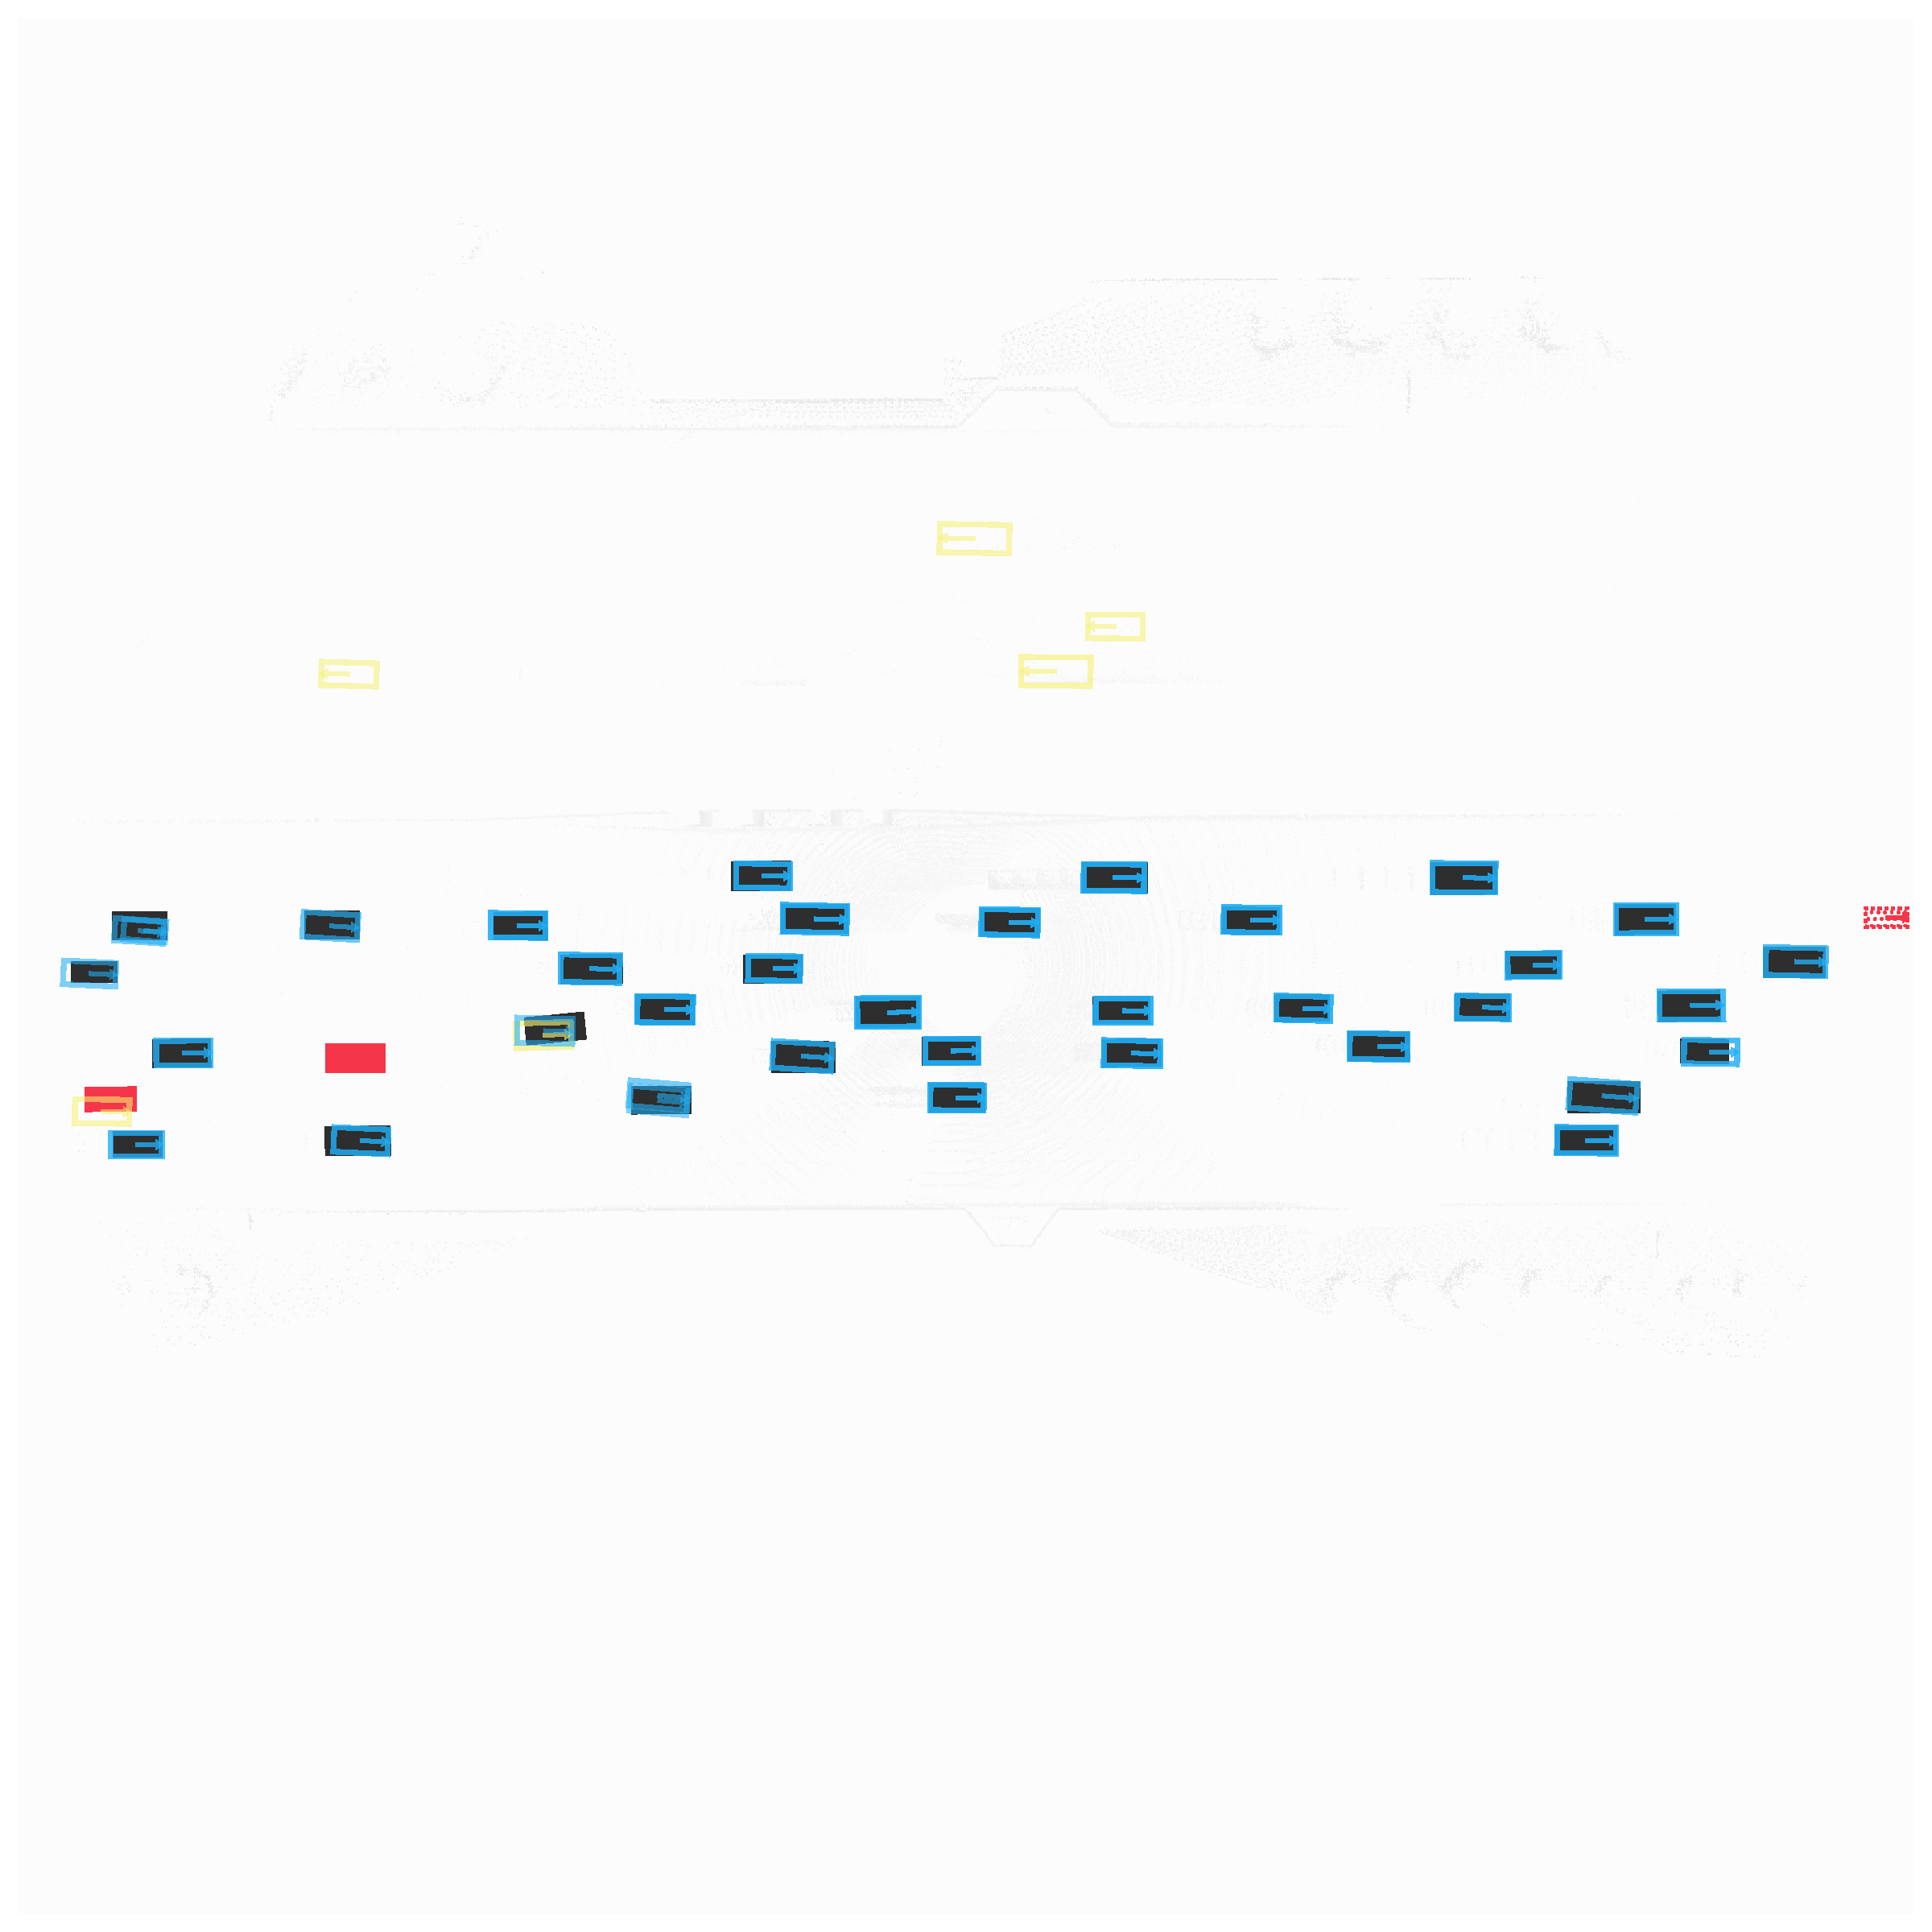
\includegraphics[width=\imw, viewport=10 270 480 740, clip]{images/images_for_supp/82/detections_wod_viz_82_120.pdf}};

        %                                                                                                                       % 72 288 936 1152
        \node[draw=black,very thick,anchor=north , inner sep=0pt]  (S7B) at ([yshift=-\rowsep]S6B.south)                   {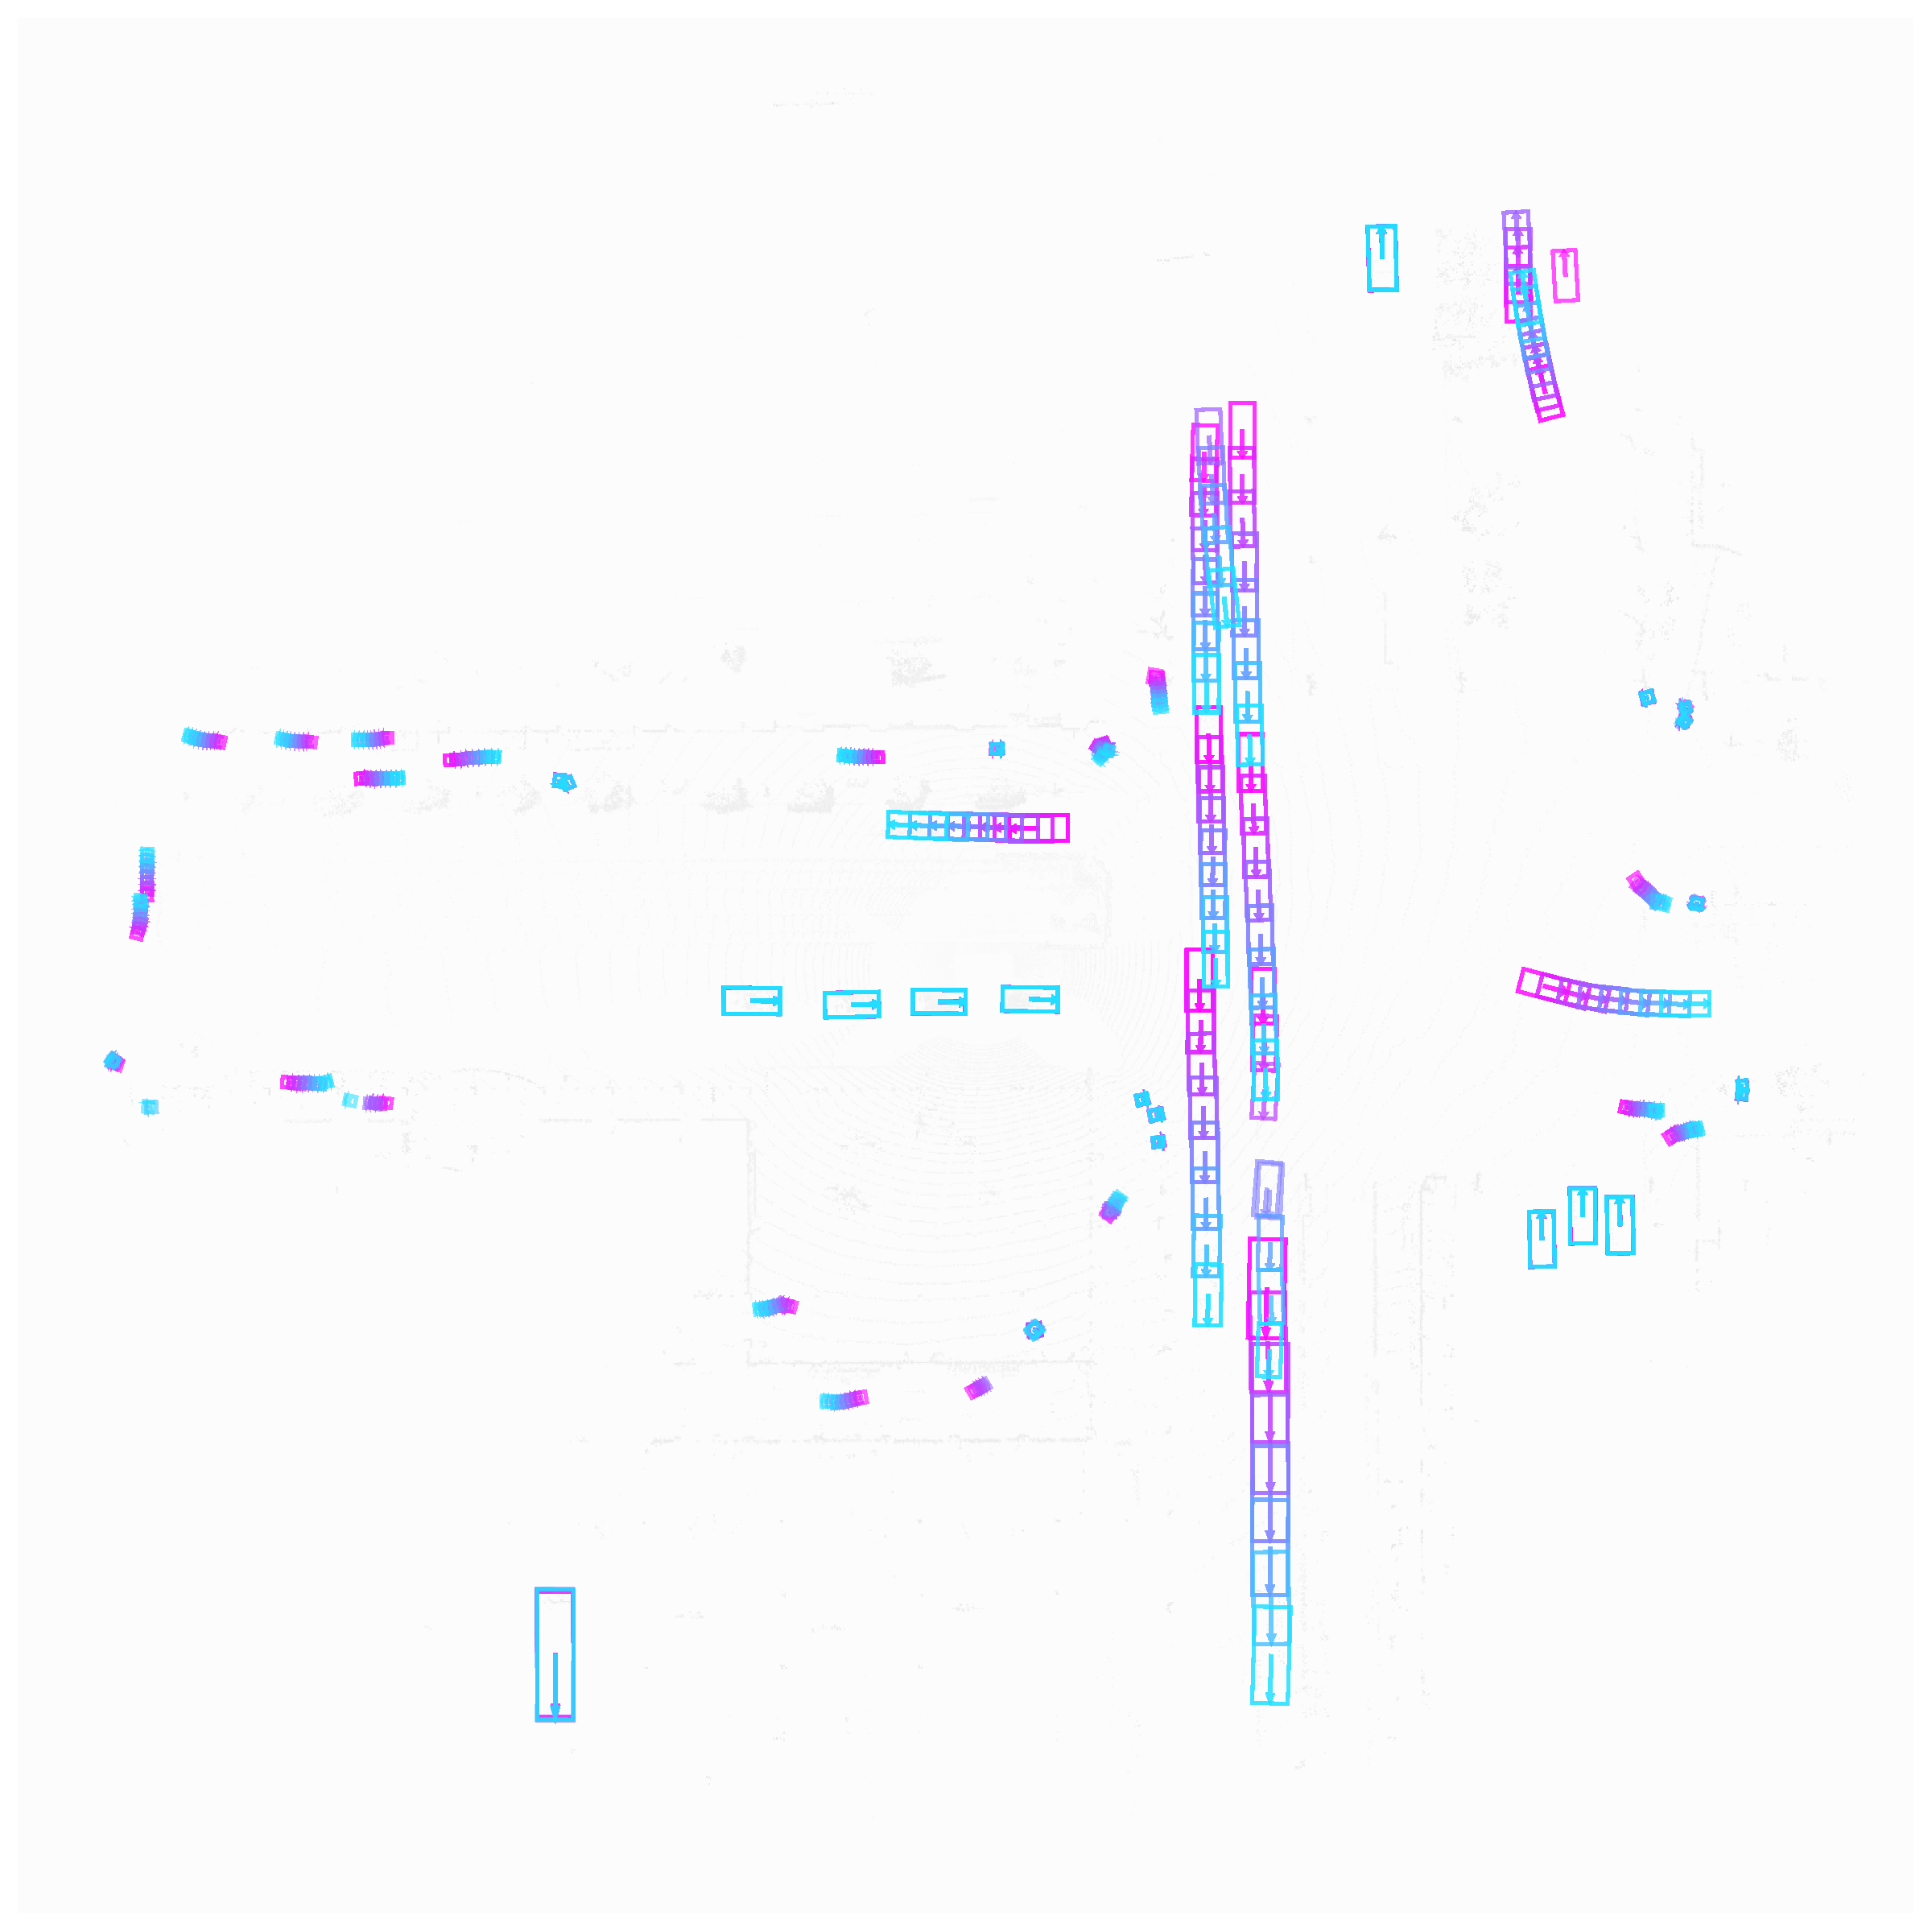
\includegraphics[width=\imw, viewport=72 72 790 790, clip]{images/images_for_supp/91/original_det_anchors_wod_viz_91_144.pdf}};
        \node[draw=black,very thick,anchor=west , inner sep=0pt]  (S7C) at (S7B.east)                   {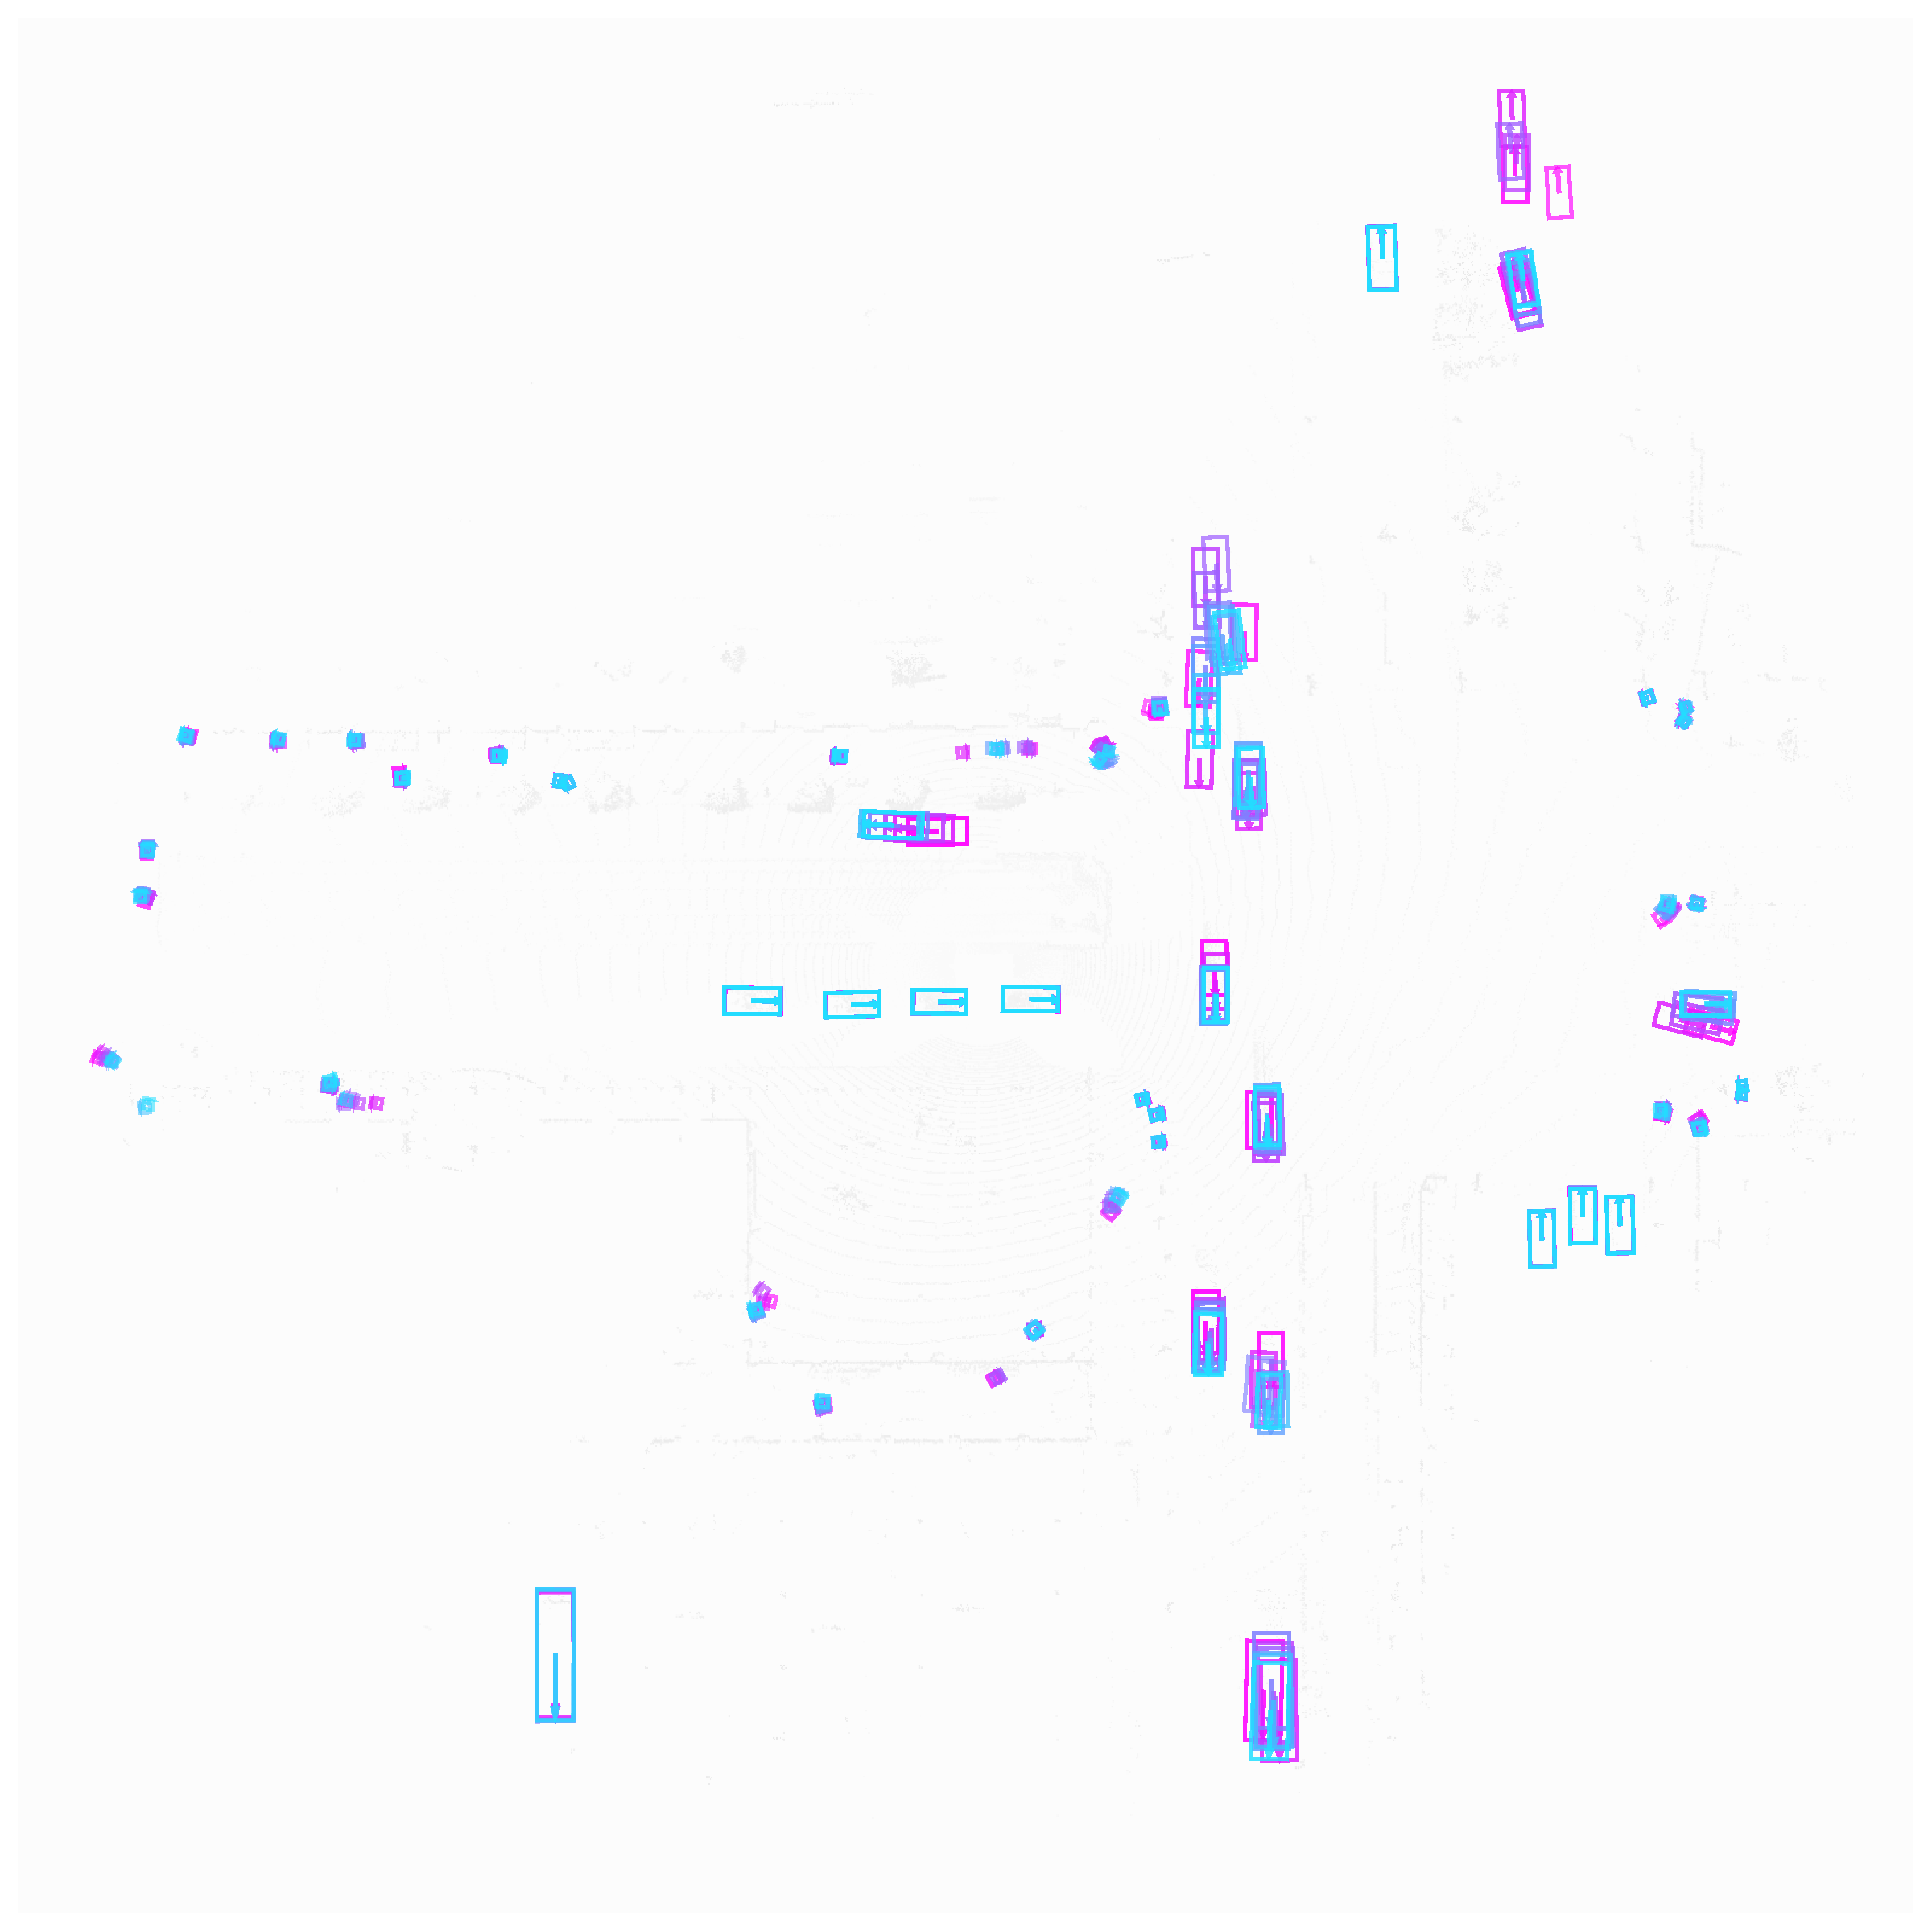
\includegraphics[width=\imw, viewport=72 72 790 790, clip]{images/images_for_supp/91/interpolated_det_anchors_wod_viz_91_144.pdf}};
        \node[draw=black,very thick,anchor=west, inner sep=0pt] (S7A) at (S7C.east) {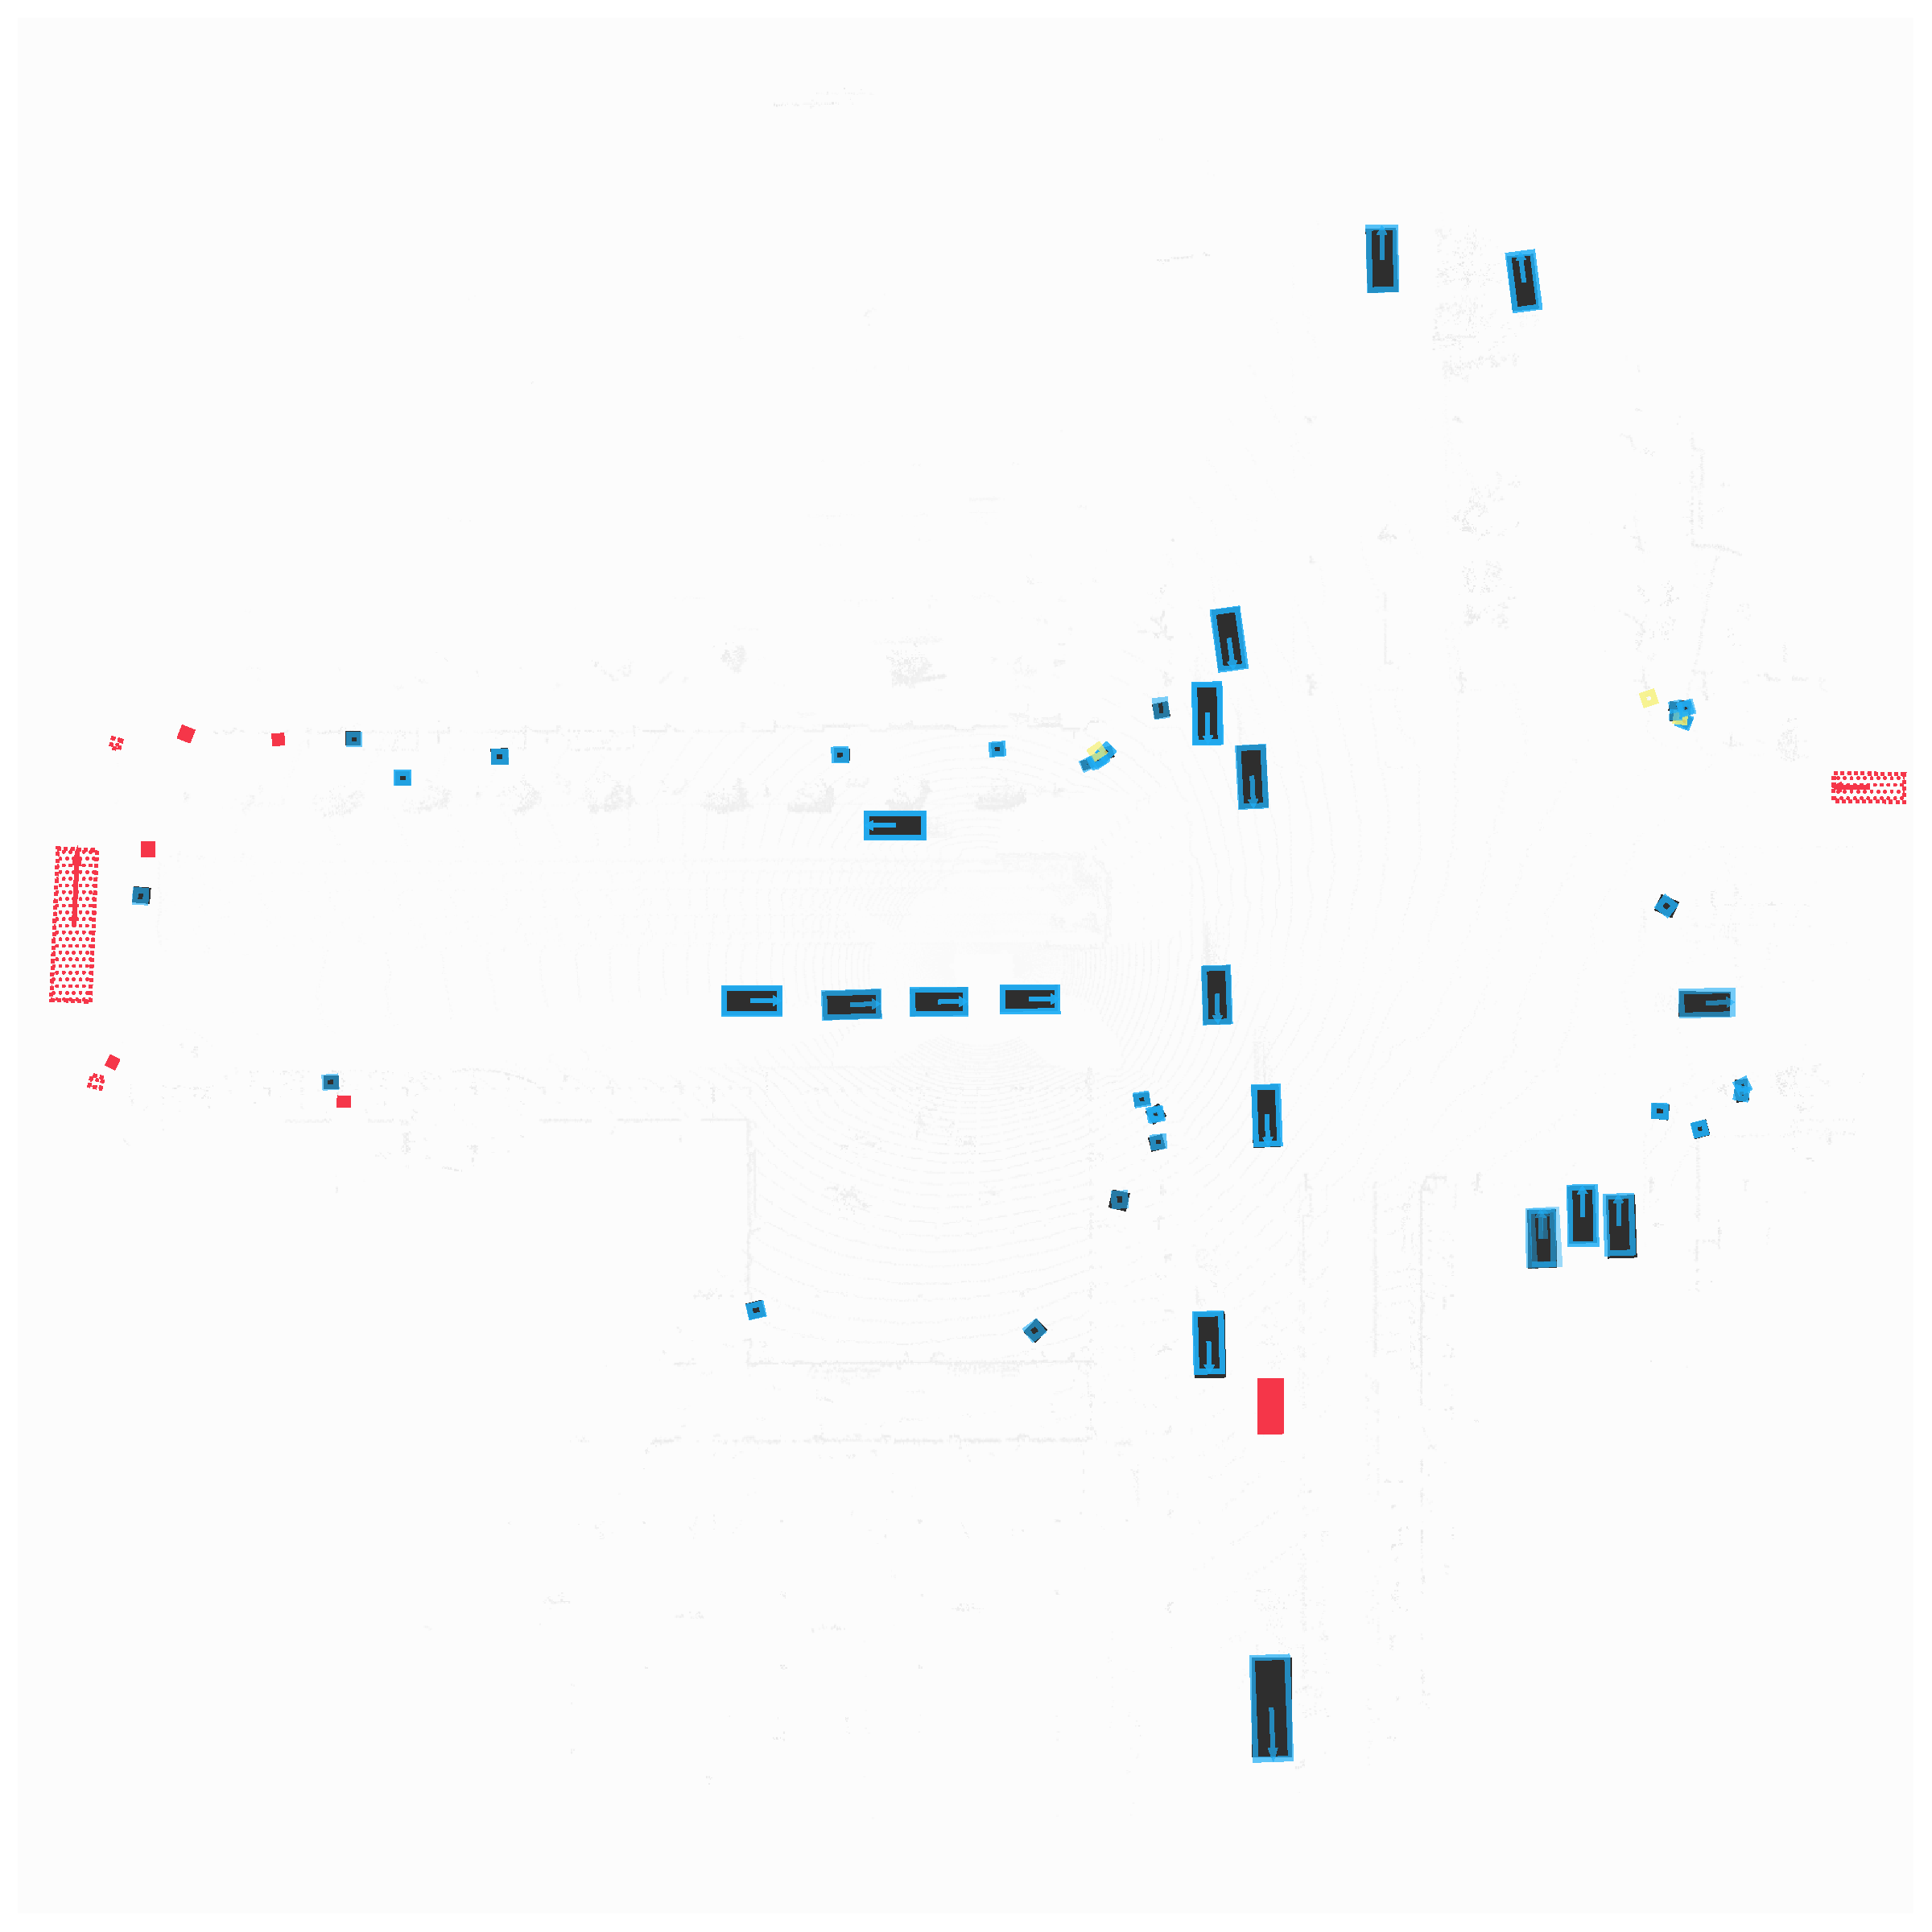
\includegraphics[width=\imw,  viewport=72 72 790 790, clip]{images/images_for_supp/91/lidar_proposals_wod_viz_91_144.pdf}};
        \node[draw=black,very thick,anchor=west , inner sep=0pt]  (S7D) at (S7A.east)                   {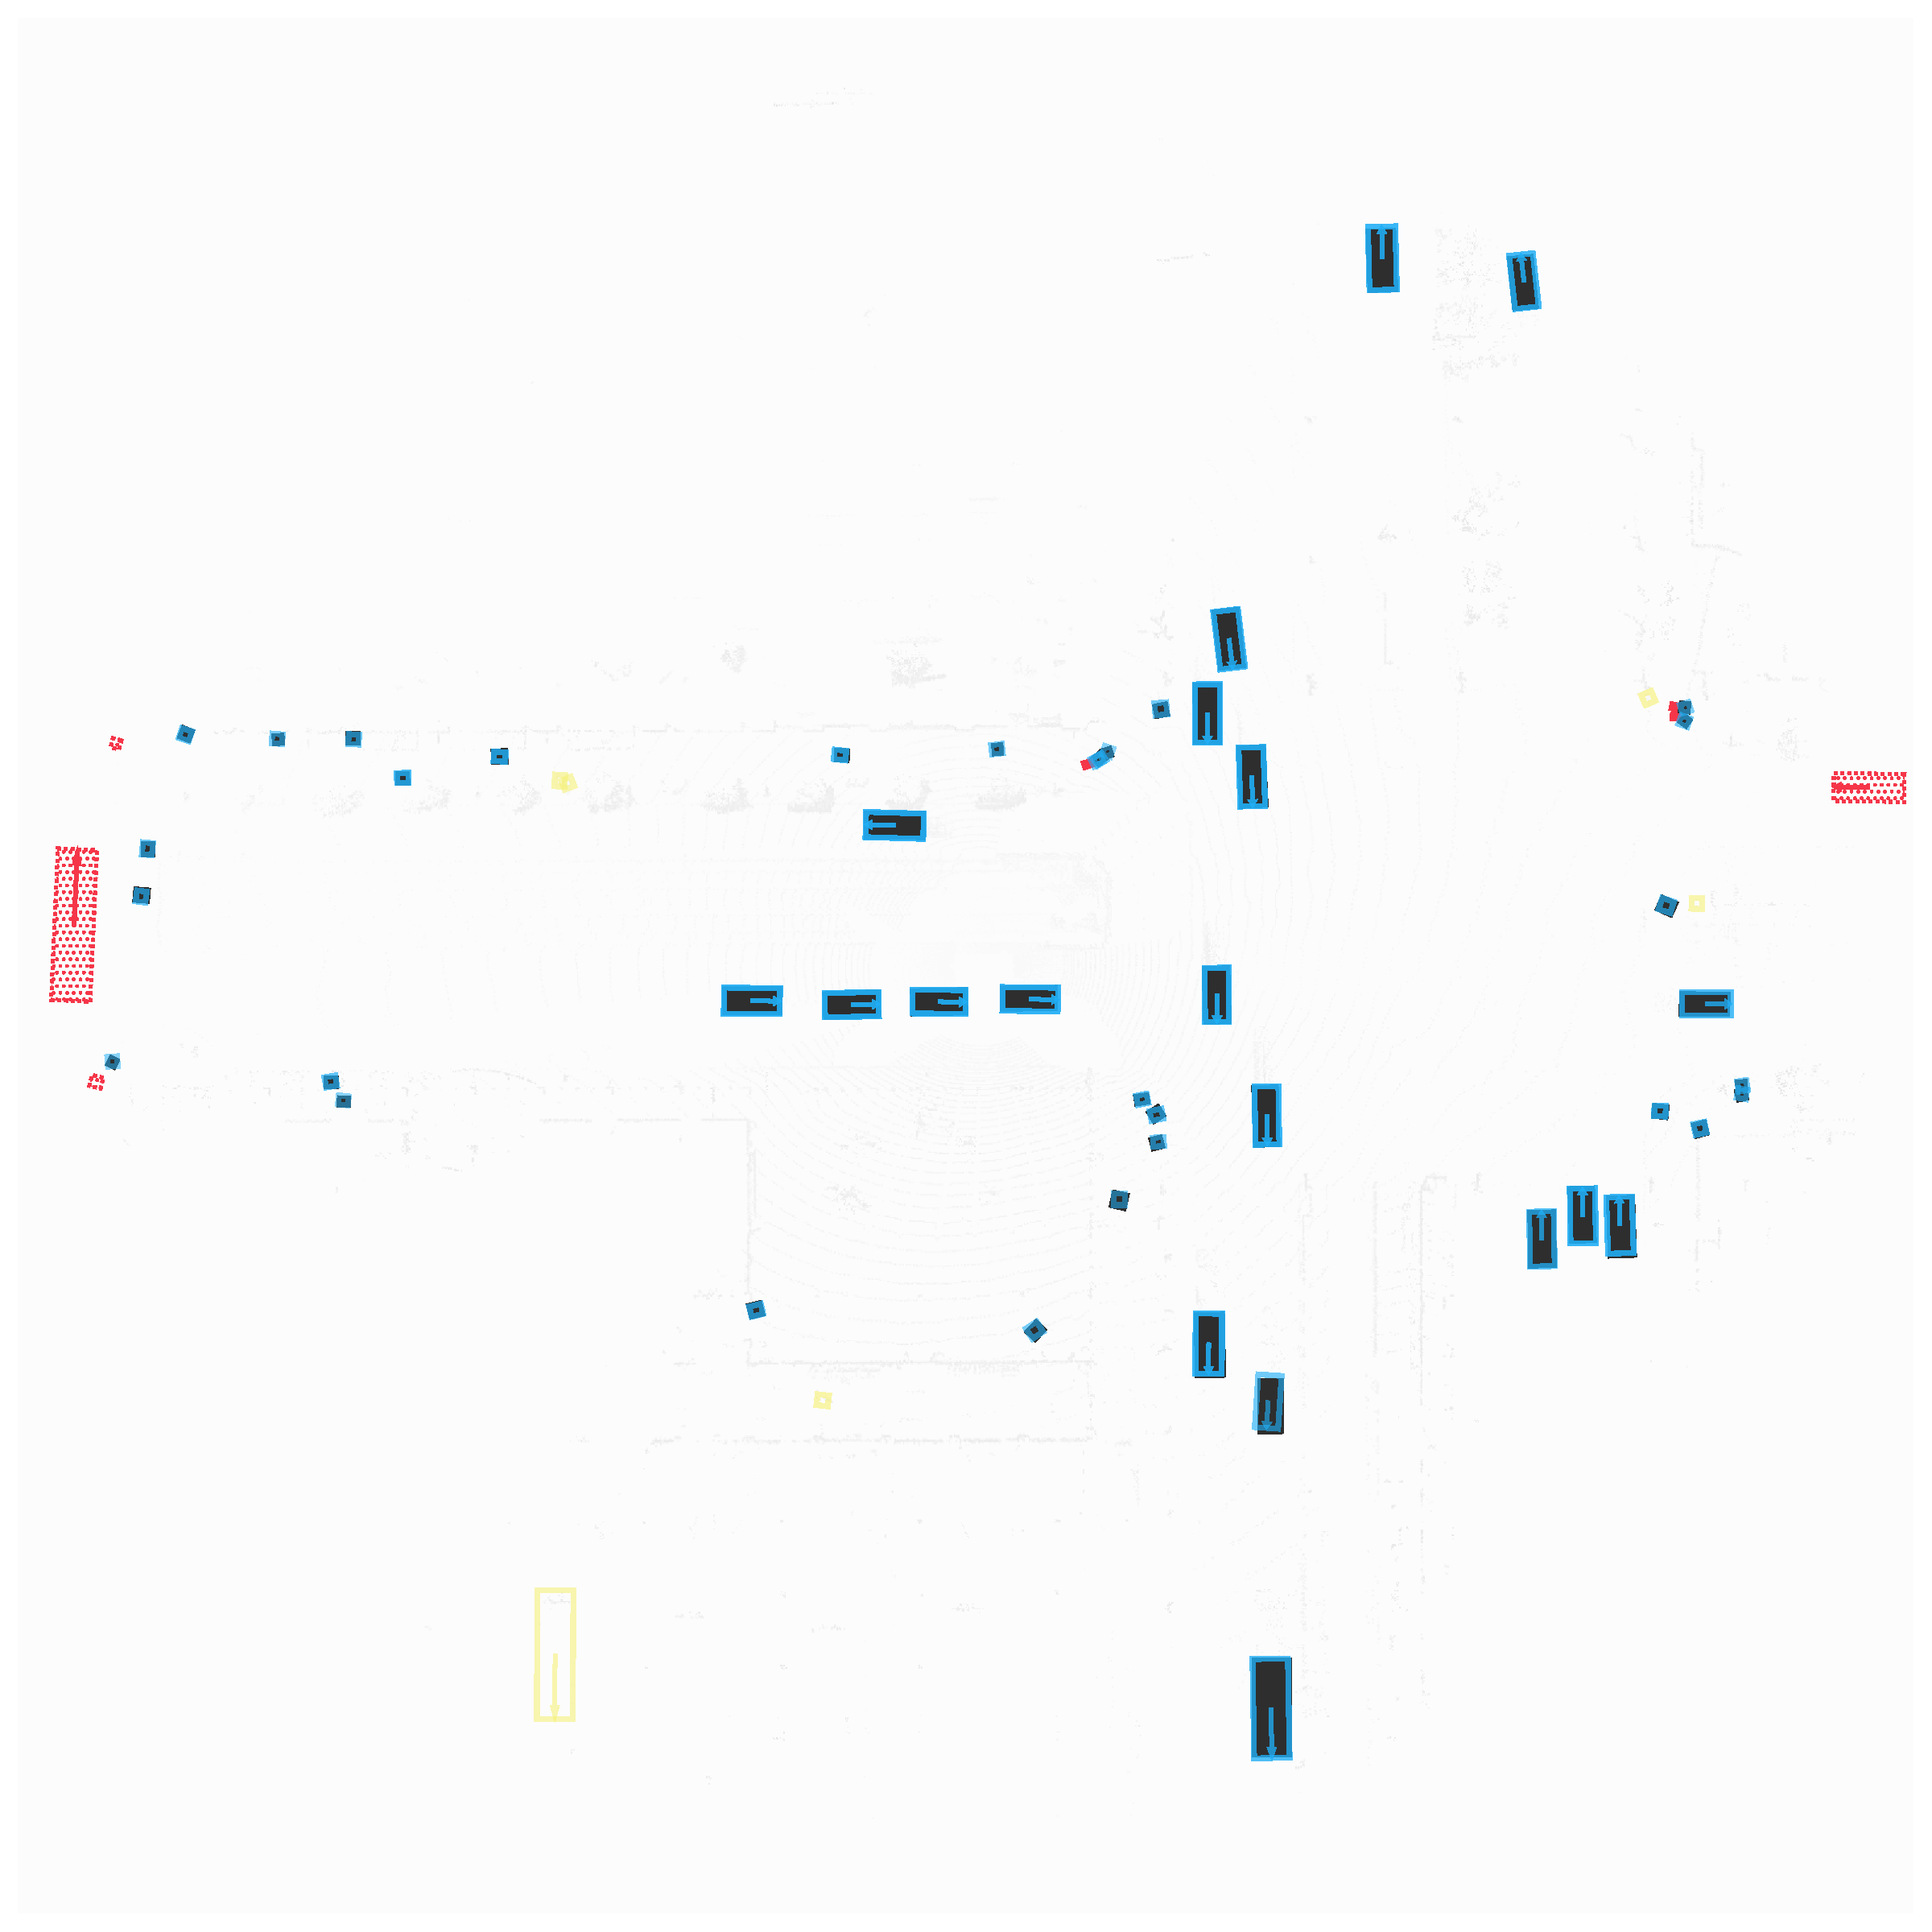
\includegraphics[width=\imw, viewport=72 72 790 790, clip]{images/images_for_supp/91/detections_wod_viz_91_144.pdf}};

        \node[draw=black,very thick,anchor=north , inner sep=0pt]  (S8B) at ([yshift=-\rowsep]S7B.south)                   {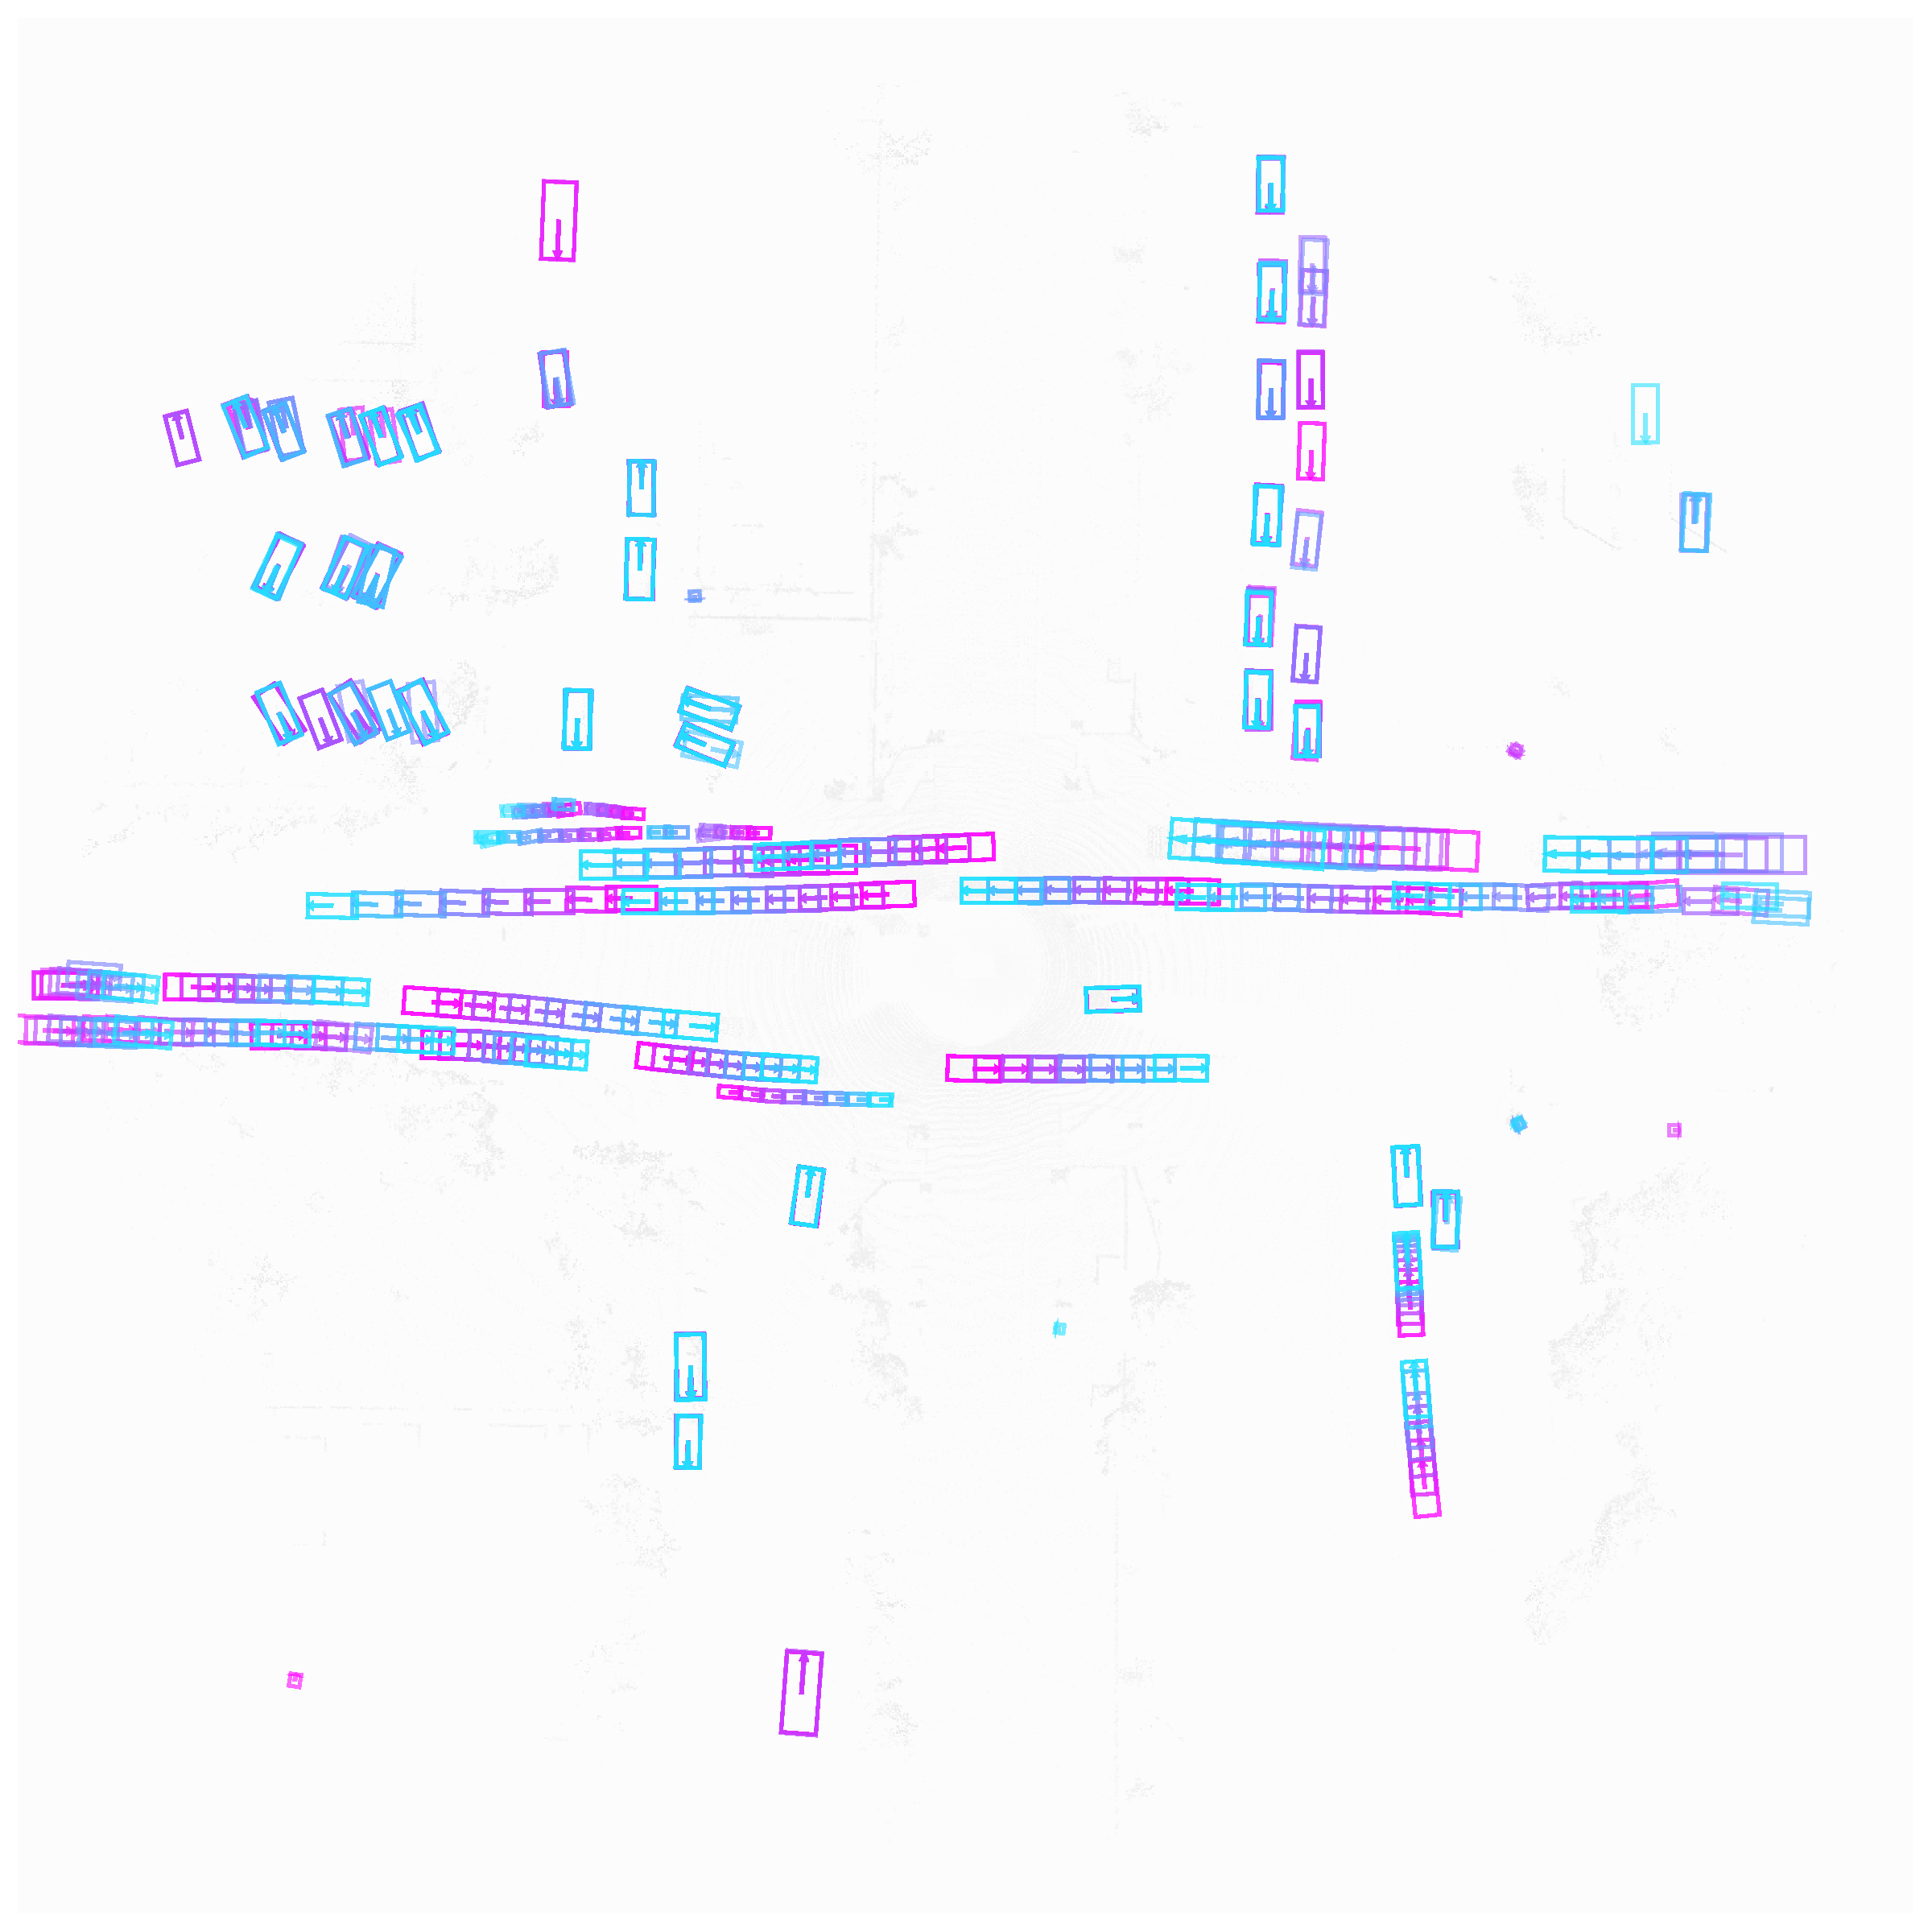
\includegraphics[width=\imw, viewport=50 360 820 1130, clip]{images/images_for_supp/161/original_det_anchors_wod_viz_161_138.pdf}};
        \node[draw=black,very thick,anchor=west , inner sep=0pt]  (S8C) at (S8B.east)                   {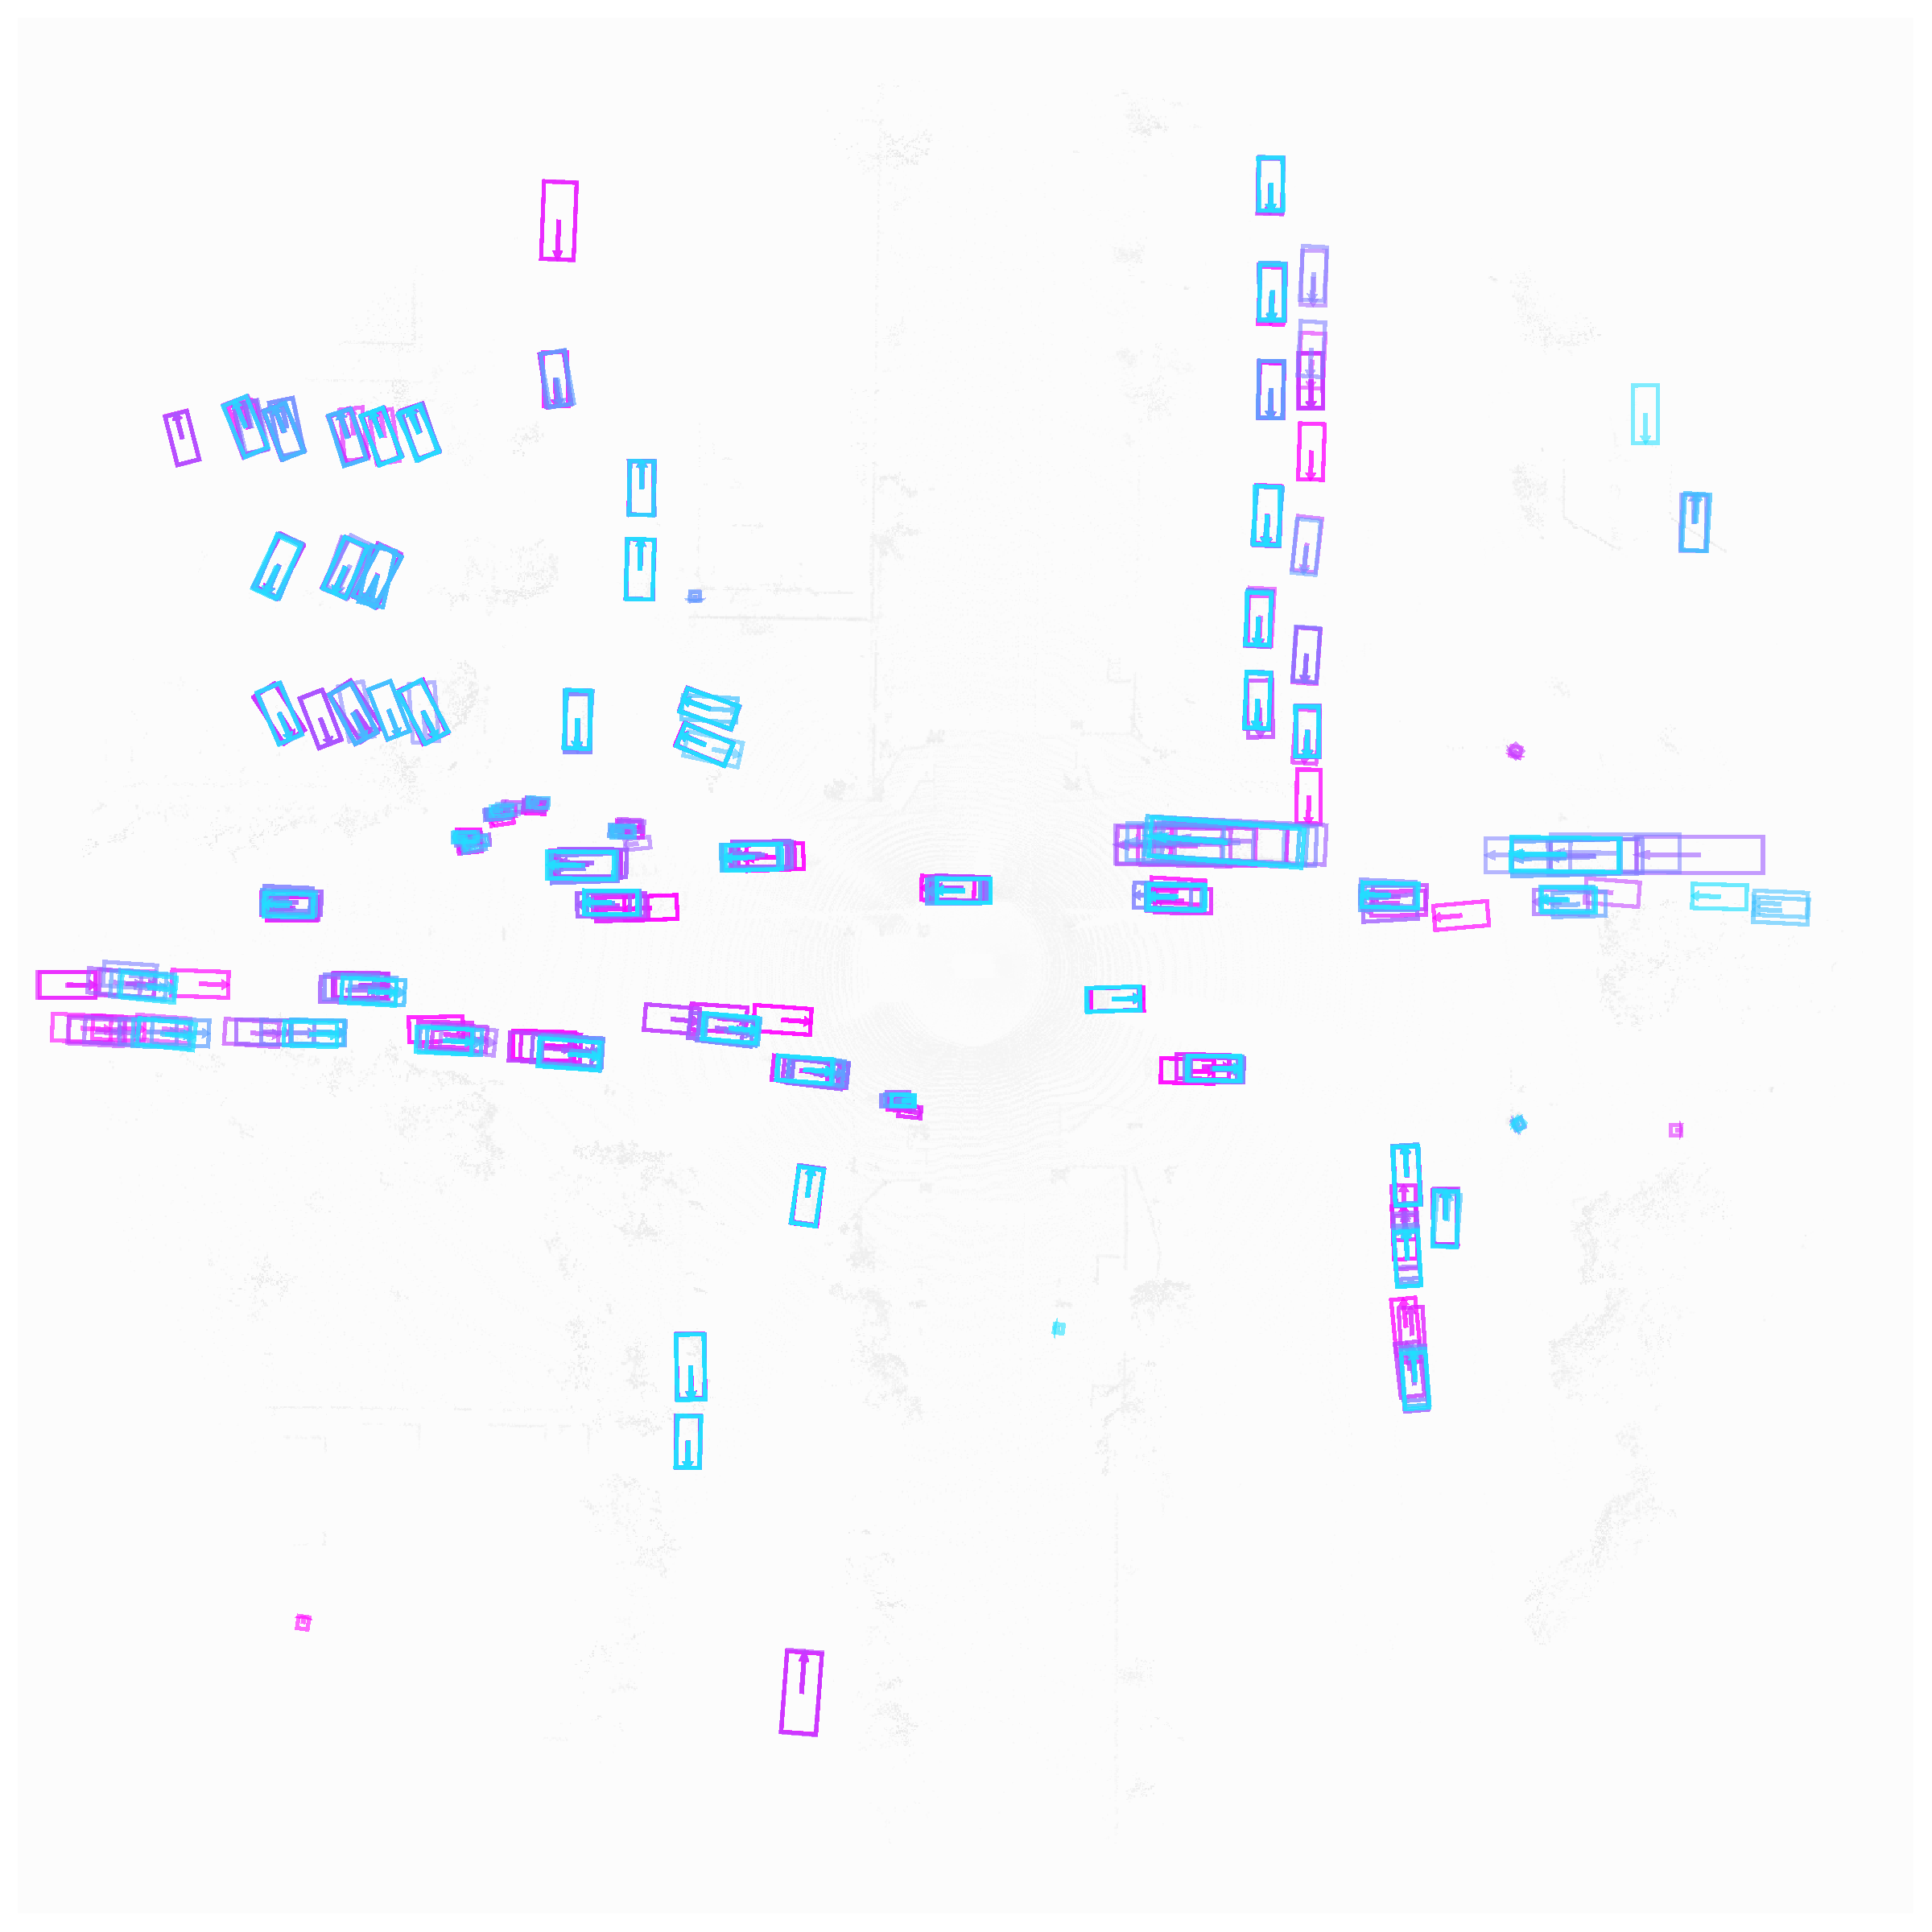
\includegraphics[width=\imw, viewport=50 360 820 1130, clip]{images/images_for_supp/161/interpolated_det_anchors_wod_viz_161_138.pdf}};
        \node[draw=black,very thick,anchor=west, inner sep=0pt] (S8A) at (S8C.east) {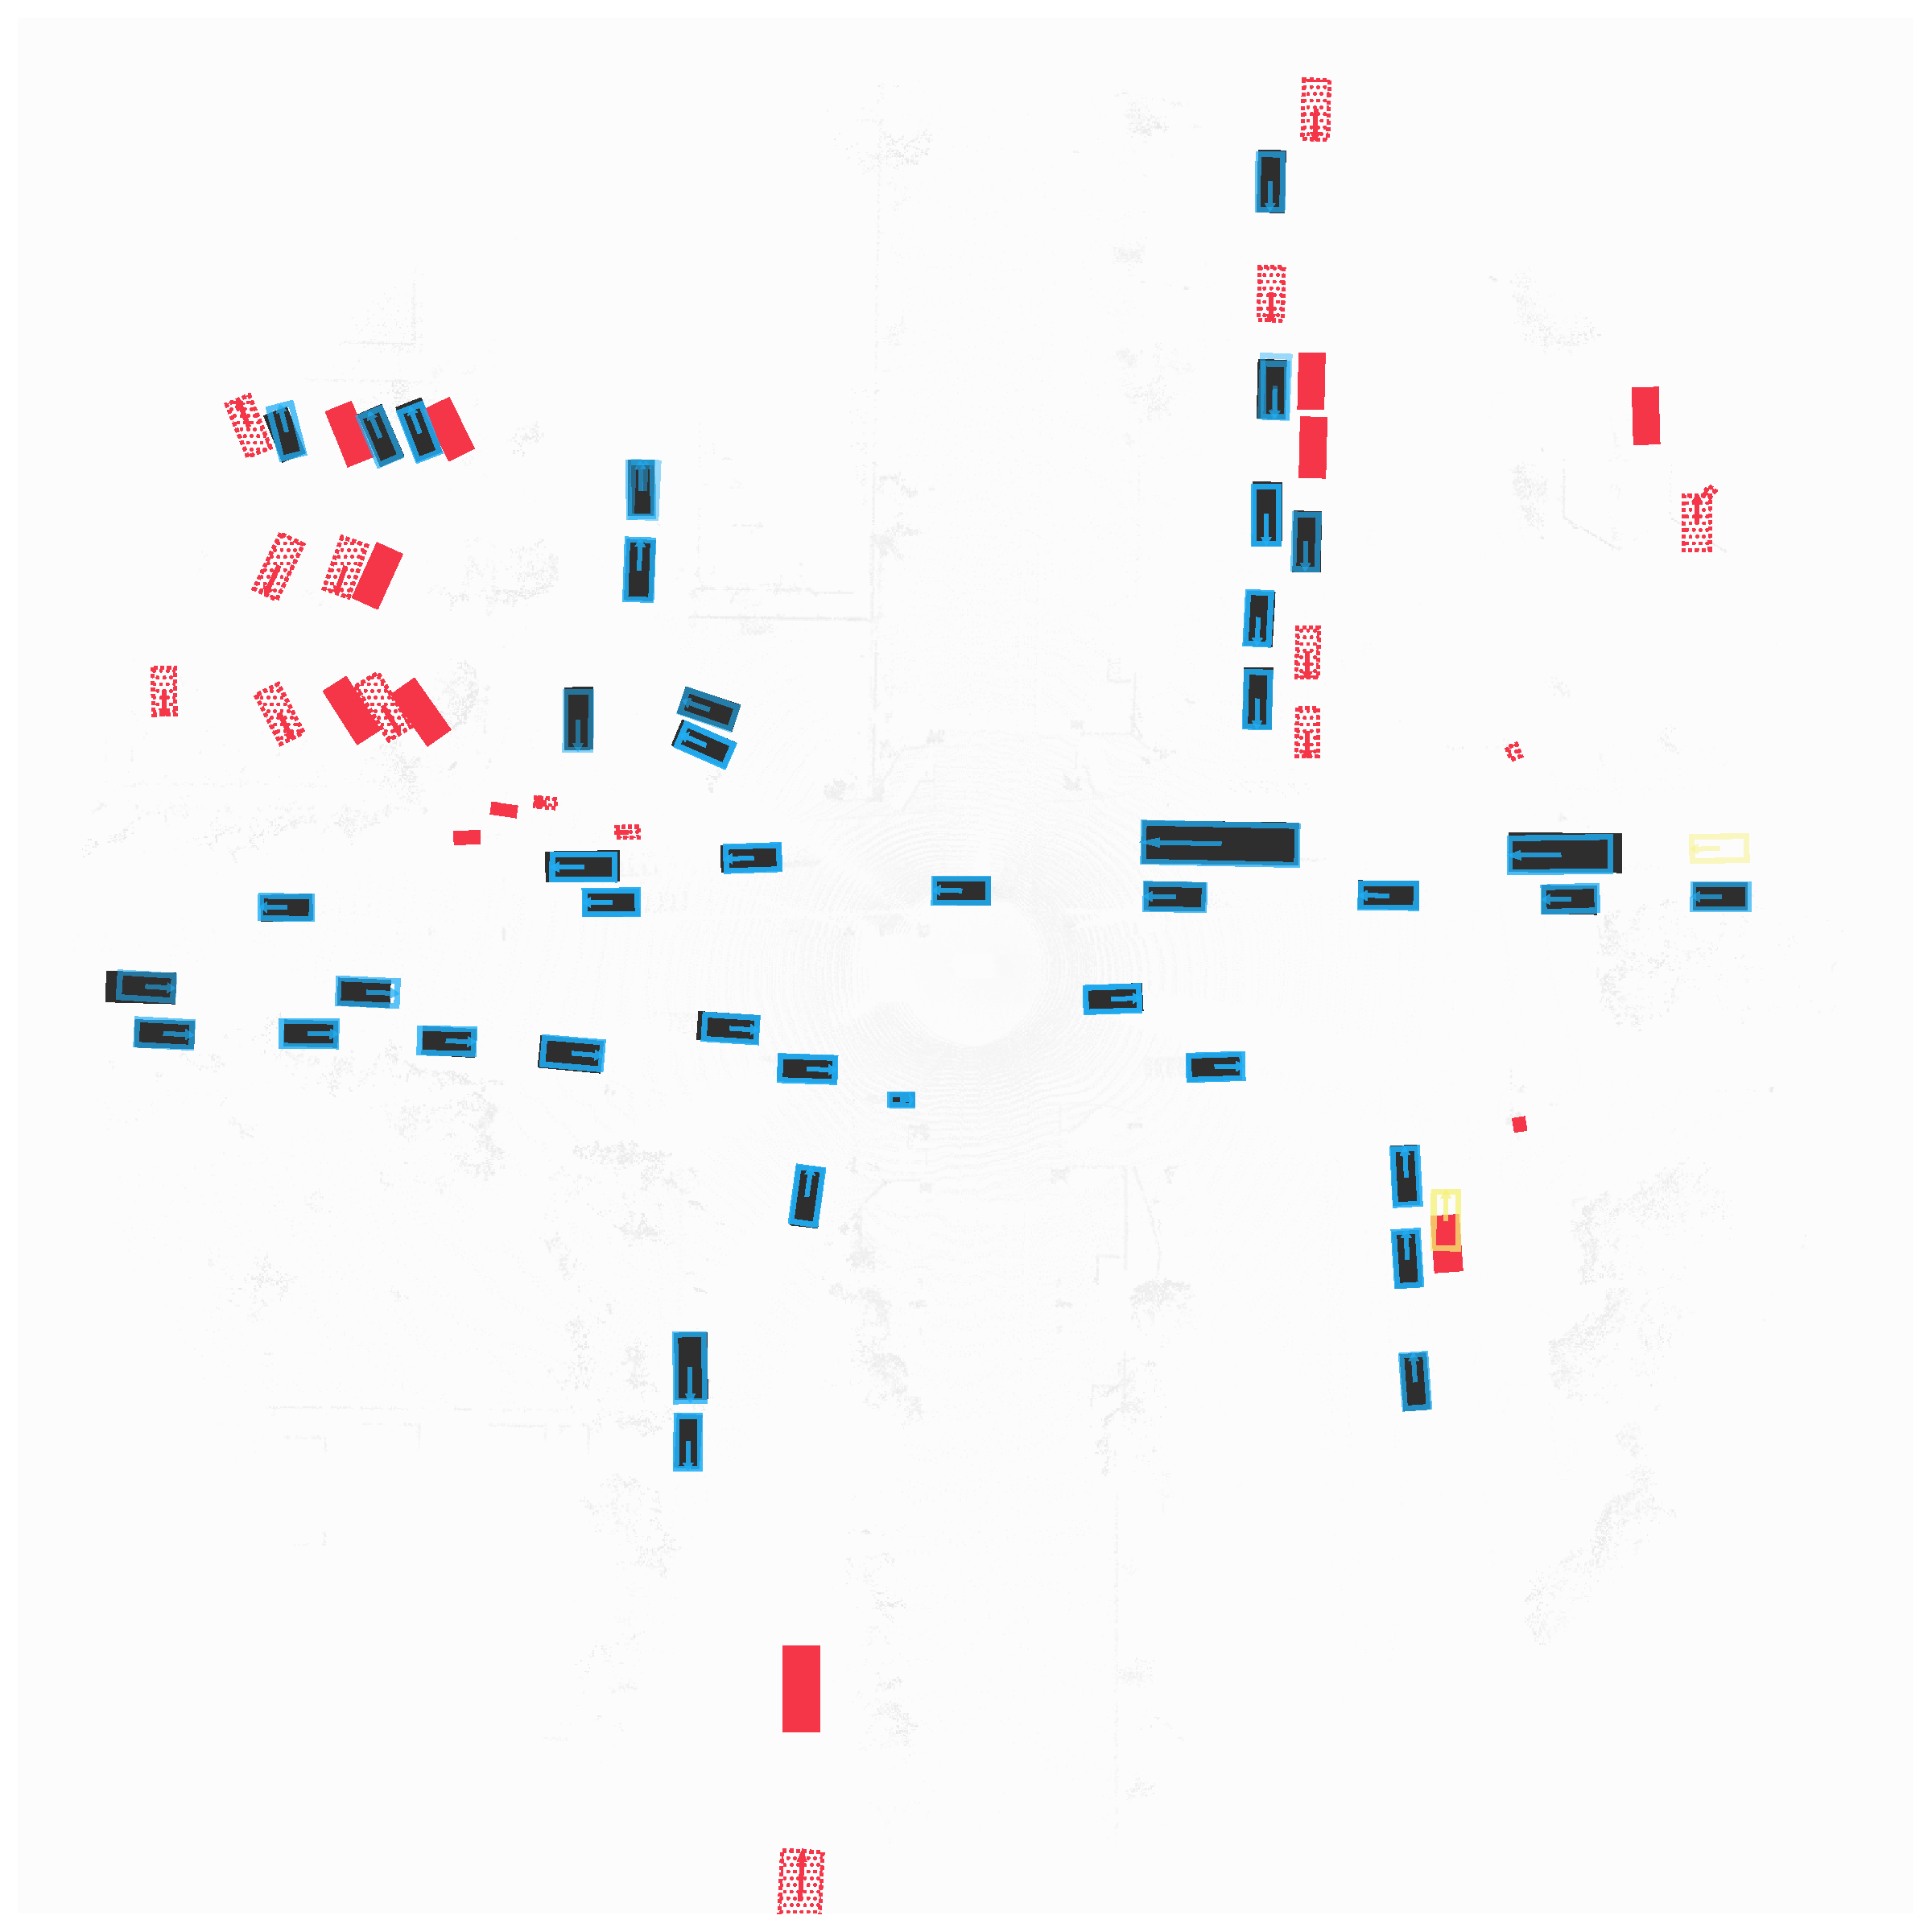
\includegraphics[width=\imw,  viewport=50 360 820 1130, clip]{images/images_for_supp/161/lidar_proposals_wod_viz_161_138.pdf}};
        \node[draw=black,very thick,anchor=west , inner sep=0pt]  (S8D) at (S8A.east)                   {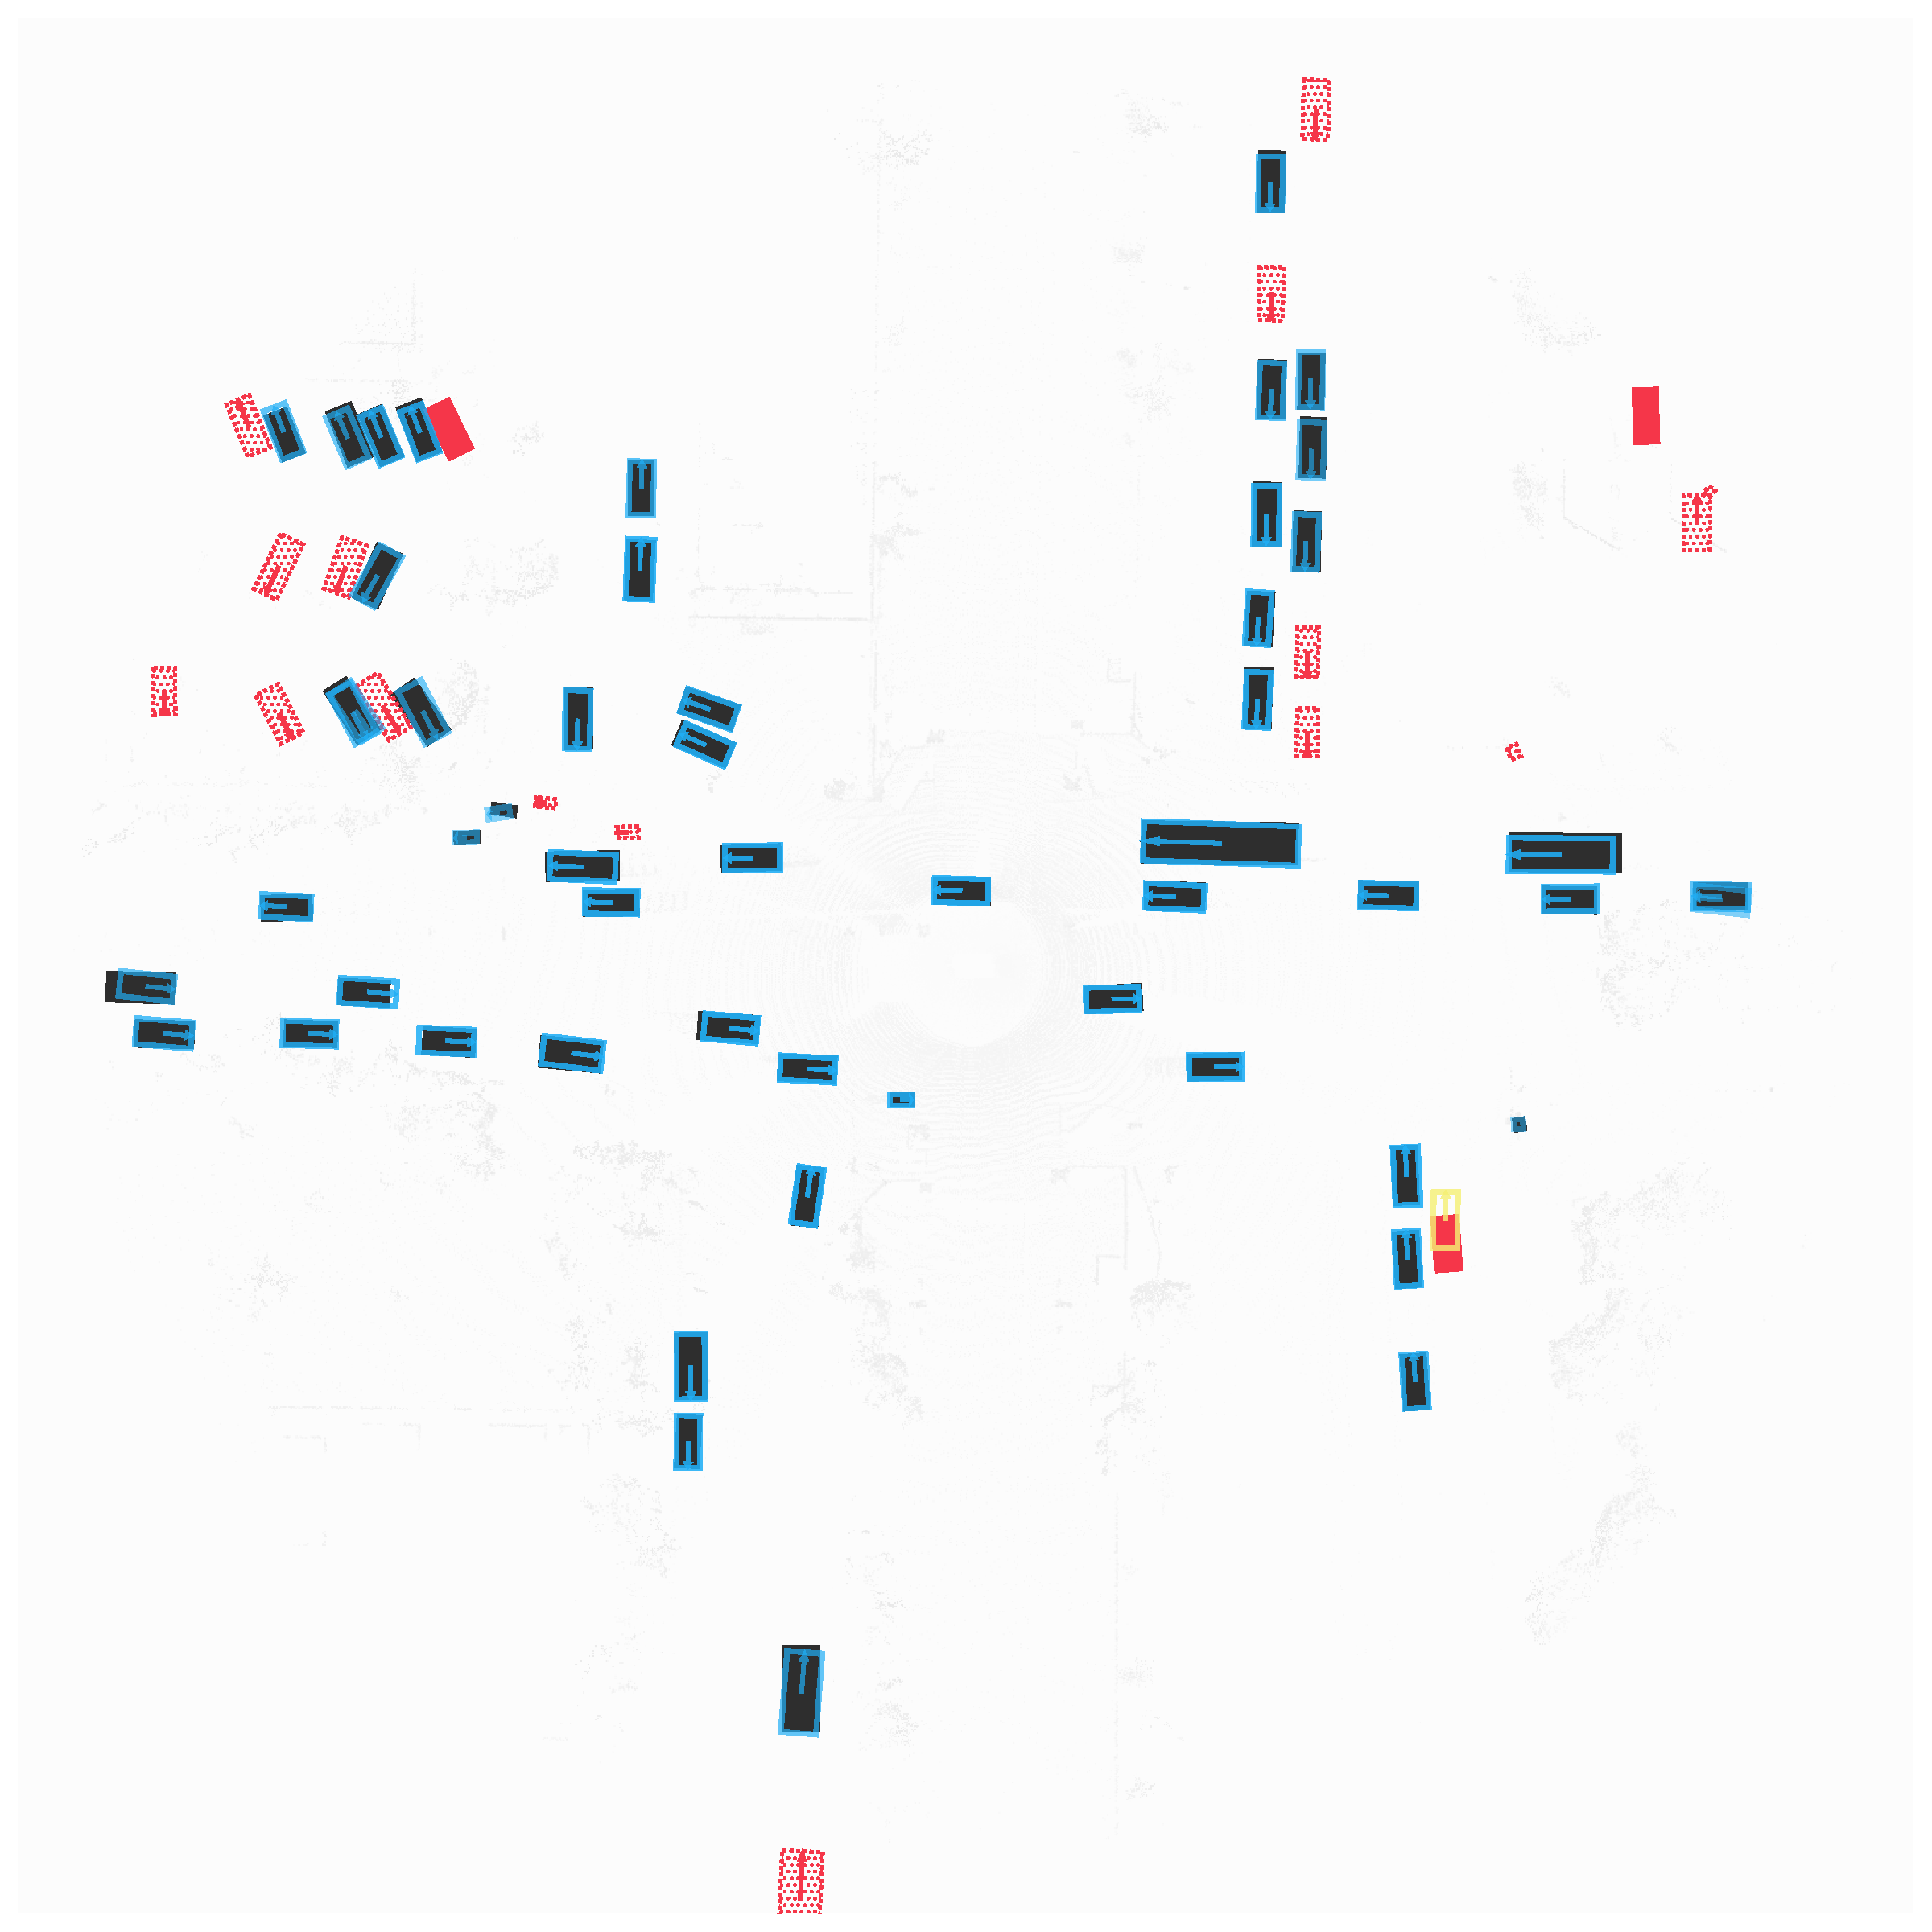
\includegraphics[width=\imw, viewport=50 360 820 1130, clip]{images/images_for_supp/161/detections_wod_viz_161_138.pdf}};
    
        % Labels for rows (Scenes)
        \node[anchor=south,rotate=90] at (S5B.west) {\footnotesize Scene \#5};
        \node[anchor=south,rotate=90] at (S6B.west) {\footnotesize Scene \#6};
        \node[anchor=south,rotate=90] at (S7B.west) {\footnotesize Scene \#7};
        \node[anchor=south,rotate=90] at (S8B.west) {\footnotesize Scene \#8};

        % colormap
        \node[inner sep=0pt,anchor=north] (cmap) at ($(S5B.north)+(0,-0.2em)$)
            {
\includegraphics[width=0.22\textwidth, height=0.8em, trim={2mm, 2mm, 2mm, 2mm}, clip, angle=180]{images/images_for_hook_light/cool_colormap.png}};
        \node[inner sep=0pt,anchor=east] (0) at ([xshift=-0.1em]cmap.east) {\footnotesize 0.0s};
        \node[inner sep=0pt,anchor=west] (1) at ([xshift=0.1em]cmap.west) {\footnotesize -2.4s};
        \node[inner sep=0pt,anchor=center] (2) at (cmap) {\footnotesize Age $(t_m - t)$};
    
        \node[inner sep=0pt,anchor=north] (cb) at ($(S5C.north)+(0,-0.2em)$)
            {
\includegraphics[width=0.22\textwidth, height=0.8em, trim={2mm, 2mm, 2mm, 2mm}, clip, angle=180]{images/images_for_hook_light/cool_colormap.png}};
        \node[inner sep=0pt,anchor=east] at ([xshift=-0.1em]cb.east) {\footnotesize 0.0s};
        \node[inner sep=0pt,anchor=west] at ([xshift=0.1em]cb.west) {\footnotesize -2.4s};
        % \node[inner sep=0pt,anchor=center] (cb.north) {\footnotesize Age $(t_m - t)$};
        

        % annotations
        \node[circle, draw=green, minimum size=0.25*\imw*2, inner sep=0pt, anchor=center, dashed] (a4) at (S5A.center) [xshift=-0.26*\imw, yshift=-0.1*\imw] {};
        \node[circle, fill=green, minimum size=0.05*\imw, inner sep=0pt] at (a4.-45) {\scriptsize{a}};
        \node[circle, fill=green, minimum size=0.05*\imw, inner sep=0pt] at (a4.-60) {\scriptsize{d}};
        \node[circle, draw=green, minimum size=0.25*\imw*2, inner sep=0pt, anchor=center, dashed] (a4b) at (S5D.center) [xshift=-0.26*\imw, yshift=-0.1*\imw] {};
        \node[circle, fill=green, minimum size=0.05*\imw, inner sep=0pt] at (a4b.-45) {\scriptsize{a}};
        \node[circle, fill=green, minimum size=0.05*\imw, inner sep=0pt] at (a4b.-60) {\scriptsize{d}};

        \node[circle, draw=green, minimum size=0.12*\imw*2, inner sep=0pt, anchor=center, dashed] (b3) at (S5A.center) [xshift=0.42*\imw, yshift=-0.22*\imw] {};
        \node[circle, fill=green, minimum size=0.05*\imw, inner sep=0pt] at (b3.-135) {\scriptsize{b}};
        \node[circle, draw=green, minimum size=0.12*\imw*2, inner sep=0pt, anchor=center, dashed] (b3b) at (S5D.center) [xshift=0.42*\imw, yshift=-0.22*\imw] {};
        \node[circle, fill=green, minimum size=0.05*\imw, inner sep=0pt] at (b3b.-135) {\scriptsize{b}};
        \node[circle, draw=green, minimum size=0.12*\imw*2, inner sep=0pt, anchor=center, dashed] (c3) at (S5C.center) [xshift=0.4*\imw, yshift=-0.24*\imw] {};
        \node[circle, fill=green, minimum size=0.05*\imw, inner sep=0pt] at (c3.-135) {\scriptsize{c}};

        \node[circle, draw=green, minimum size=0.15*\imw*2, inner sep=0pt, anchor=center, dashed] (b4) at (S6A.center) [xshift=0.22*\imw, yshift=-0.0*\imw] {};
        \node[circle, fill=green, minimum size=0.05*\imw, inner sep=0pt] at (b4.-45) {\scriptsize{b}};
        \node[circle, draw=green, minimum size=0.15*\imw*2, inner sep=0pt, anchor=center, dashed] (b4b) at (S6D.center) [xshift=0.22*\imw, yshift=-0.0*\imw] {};
        \node[circle, fill=green, minimum size=0.05*\imw, inner sep=0pt] at (b4b.-45) {\scriptsize{b}};

        \node[circle, draw=green, minimum size=0.1*\imw*2, inner sep=0pt, anchor=center, dashed] (c4) at (S6C.center) [xshift=0.2*\imw, yshift=0.07*\imw] {};
        \node[circle, fill=green, minimum size=0.05*\imw, inner sep=0pt] at (c4.-45) {\scriptsize{c}};

        \node[circle, draw=green, minimum size=0.08*\imw*2, inner sep=0pt, anchor=center, dashed] (b5) at (S7A.center) [xshift=0.46*\imw, yshift=-0.17*\imw] {};
        \node[circle, fill=green, minimum size=0.05*\imw, inner sep=0pt] at (b5.-135) {\scriptsize{b}};
        \node[circle, draw=green, minimum size=0.08*\imw*2, inner sep=0pt, anchor=center, dashed] (b5b) at (S7D.center) [xshift=0.46*\imw, yshift=-0.17*\imw] {};
        \node[circle, fill=green, minimum size=0.05*\imw, inner sep=0pt] at (b5b.-135) {\scriptsize{b}};
        \node[circle, draw=green, minimum size=0.08*\imw*2, inner sep=0pt, anchor=center, dashed] (c5) at (S7C.center) [xshift=0.46*\imw, yshift=-0.17*\imw] {};
        \node[circle, fill=green, minimum size=0.05*\imw, inner sep=0pt] at (c5.-135) {\scriptsize{c}};

        \node[circle, draw=green, minimum size=0.18*\imw*2, inner sep=0pt, anchor=center, dashed] (d5) at (S7A.center) [xshift=-0.32*\imw, yshift=0.3*\imw] {};
        \node[circle, fill=green, minimum size=0.05*\imw, inner sep=0pt] at (d5.-45) {\scriptsize{d}};
        \node[circle, draw=green, minimum size=0.18*\imw*2, inner sep=0pt, anchor=center, dashed] (d5b) at (S7D.center) [xshift=-0.32*\imw, yshift=0.3*\imw] {};
        \node[circle, fill=green, minimum size=0.05*\imw, inner sep=0pt] at (d5b.-45) {\scriptsize{d}};
        \node[circle, draw=green, minimum size=0.18*\imw*2, inner sep=0pt, anchor=center, dashed] (c6) at (S7C.center) [xshift=-0.32*\imw, yshift=0.3*\imw] {};
        \node[circle, fill=green, minimum size=0.05*\imw, inner sep=0pt] at (c6.-45) {\scriptsize{c}};

        \node[circle, draw=green, minimum size=0.1*\imw*2, inner sep=0pt, anchor=center, dashed] (d6) at (S8A.center) [xshift=-0.14*\imw, yshift=-0.12*\imw] {};
        \node[circle, fill=green, minimum size=0.05*\imw, inner sep=0pt] at (d6.-45) {\scriptsize{d}};
        \node[circle, draw=green, minimum size=0.1*\imw*2, inner sep=0pt, anchor=center, dashed] (d6b) at (S8D.center) [xshift=-0.14*\imw, yshift=-0.12*\imw] {};
        \node[circle, fill=green, minimum size=0.05*\imw, inner sep=0pt] at (d6b.-45) {\scriptsize{d}};
        \node[circle, draw=green, minimum size=0.1*\imw*2, inner sep=0pt, anchor=center, dashed] (c7) at (S8C.center) [xshift=-0.14*\imw, yshift=-0.12*\imw] {};
        \node[circle, fill=green, minimum size=0.05*\imw, inner sep=0pt] at (c7.-45) {\scriptsize{c}};

        \node[circle, draw=green, minimum size=0.2*\imw*2, inner sep=0pt, anchor=center, dashed] (a5) at (S8A.center) [xshift=-0.27*\imw, yshift=0.1*\imw] {};
        \node[circle, fill=green, minimum size=0.05*\imw, inner sep=0pt] at (a5.45) {\scriptsize{a}};
        \node[circle, draw=green, minimum size=0.2*\imw*2, inner sep=0pt, anchor=center, dashed] (a5b) at (S8D.center) [xshift=-0.27*\imw, yshift=0.1*\imw] {};
        \node[circle, fill=green, minimum size=0.05*\imw, inner sep=0pt] at (a5b.45) {\scriptsize{a}};

        \node[circle, draw=green, minimum size=0.1*\imw*2, inner sep=0pt, anchor=center, dashed] (a6) at (S8A.center) [xshift=0.43*\imw, yshift=0.22*\imw] {};
        \node[circle, fill=green, minimum size=0.05*\imw, inner sep=0pt] at (a6.45) {\scriptsize{a}};
        \node[circle, draw=green, minimum size=0.1*\imw*2, inner sep=0pt, anchor=center, dashed] (a6b) at (S8D.center) [xshift=0.43*\imw, yshift=0.22*\imw] {};
        \node[circle, fill=green, minimum size=0.05*\imw, inner sep=0pt] at (a6b.45) {\scriptsize{a}};
    
\end{tikzpicture}
\caption{Visualization of bounding box proposals of \ourmodel{} enhancing CenterPoint 1f~\cite{centerpoint} on the WOD validation set.
We threshold at the max f1 score for the detection proposals and model outputs.
Filled boxes are labels: \colorbox{gt}{\textcolor{white}{black}} are matched labels, \colorbox{red}{red} boxes are false negatives,
and dotted boxes have $< 1$ LiDAR point observation
Box outlines are predictions: \textcolor{tp}{\fbox{blue}} boxes are true positive proposals, and \textcolor{fp}{\fbox{yellow}} boxes are false positives.
Annotations which we refer to in the main text are in \textcolor{green}{green}.
For computing the matching boxes in visualization, we use IoU thresholds of 0.5, 0.1, and 0.1 for Veh., Ped., and Cyc., respectively.
% \ben{TODO: remove arrows on pedestrians in memory}
}
\label{fig:supp-quali-2}
\end{figure*}